\section{Numerical Results} \label{chap:NuRe:1}
In this section, we illustrate the performance of the greedy generation of a symplectic basis. First, the parametric linear wave equation is considered to compare SVD based methods with the greedy method. The nonlinear model order reduction using the combination of DIEM and the symplectic basis is then illustrated by considering the parametric nonlinear Schr\"odinger equation.

\subsection{Parametric Linear Wave equation} Consider the {\edit parametric} linear wave equation
\begin{equation} \label{eq:NuRe:1}
\left\{
\begin{aligned}
& u_{tt}(x,t,\omega) = \kappa(\omega) u_{xx}(x,t,\omega), \\
& u(x,0) = u^0(x),
\end{aligned}
\right.
\end{equation}
where $x$ belongs to a one-dimensional torus of length $L$, $\omega = (\omega_1,\dots,\omega_4)$ and
\begin{equation} \label{eq:NuRe:2}
	\kappa(\omega) = c^2\left( \sum_{l=1}^4 \frac{1}{l^2} \omega_l \right).
\end{equation}
Each $\omega_l$ is uniformly distributed in $[0,1]$ and $c\in \mathbb{R}$ is a constant number. By rewriting (\ref{eq:NuRe:1}) in canonical form, using the change of variable $q = u$ and $\partial q/ \partial t= p$, we obtain the symplectic form
\begin{equation} \label{eq:NuRe:3}
\left\{
\begin{aligned}
& q_t(x,t,\omega) = p(x,t,\omega), \\
& p_t(x,t,\omega) = \kappa(\omega) q_{xx}(x,t,\omega),
\end{aligned}
\right.
\end{equation}
with the associated Hamiltonian given by
\begin{equation} \label{eq:NuRe:4}
	H(q,p,\omega) = \frac 1 2 \int_0^L p^2 + \kappa(\omega) q_x^2 \ dx.
\end{equation}
We discretized the torus into $N$ equidistant points and define $\Delta x = L/N$, $x_i = i\Delta x$, $q_i=q(t,x_i,\omega)$ and $p_i=p(t,x_i,\omega)$ for $i = 1, \dots, N$. Furthermore, we discretize (\ref{eq:NuRe:3}) using a standard central finite differences scheme to obtain
\begin{equation} \label{eq:NuRe:5}
	\frac{d}{dt} \mathbf z = \mathbb{J}_{2N} L\mathbf z,
\end{equation}
where $\mathbf z=(q,\dots,q_N,p_q,\dots,p_n)^T$ and
\begin{equation} \label{eq:NuRe:6}
L = 
\begin{pmatrix}
	I_n & 0_N \\
	0_N & \kappa(\omega)D_{xx}
\end{pmatrix},\quad 
\end{equation}
with $D_{xx}$ the central finite differences matrix operator. The discrete Hamiltonian can finally be written as
\begin{equation} \label{eq:NuRe:7}
	H_{\Delta x}(\mathbf z) = \frac{\Delta x}2 \sum_{i=1}^{N} \left( p_i^2 + \kappa(\omega) \frac{(q_{i+1} - q_i)^2}{2\Delta x ^ 2} + \kappa(\omega) \frac{(q_{i} - q_{i-1})^2}{2\Delta x ^ 2} \right).
\end{equation}
The initial condition is given by
\begin{equation} \label{eq:NuRe:8}
	q_i(0) = h( 10\times|x_i - \frac{1}{2}| ), \quad p_i = 0, \quad i=1,\dots,N
\end{equation}
where $h(s)$ is the cubic spline function
\begin{equation} \label{eq:NuRe:9}
h(s) = 
\left\{
\begin{aligned}
& 1 - \frac{3}{2}s^2 + \frac{3}{4}s^3, \quad & 0\leq s \leq 1, \\
& \frac{1}{4}(2-s)^3, & 1< s \leq 2, \\
& 0, & s > 2.
\end{aligned}
\right.
\end{equation}
This will result in waves propagating in both directions on the torus.

For numerical time integration we {\edit use} the Str\"omer-Verlet (\ref{eq:Hasy:13}) scheme, which becomes an explicit scheme since the Hamiltonian is separable for the linear wave-equation. The full model uses the following parameter set \vspace{0.5cm}
\begin{center}
\begin{tabular}{|l|l|}
\hline
Domain length & $L = 1$ \\
No. grid points & $N = 500$ \\
Space discretization size & $\Delta x = 0.002$ \\
Time discretization size & $\Delta t = 0.01$ \\
\hline
\end{tabular}
\end{center}
\vspace{0.5cm}

We compare the reduced system obtained by the greedy algorithm with the methods based on SVD. To generate snapshots, we discretize the parameter space $[0,1]^4$ into in total of $5^4$ equidistant grid points. For the SVD based methods and POD, snapshots are gathered in the snapshot matrices $S$, $S_{\text{combined}}$ and $S_{\text{complex}}$, respectively, and the SVD is performed to construct the reduced basis. The greedy method is applied according to Algorithm \ref{alg:SyMo:3}; as input, the tolerance for the error in the Hamiltonian is set to $\delta = 5 \times 10^{-3}$. All reduced systems are taken to have an identical size ($k=80$ for POD and $k=40$ for the symplectic methods). We use the Verlet-Str\"omer scheme for symplectic methods and a second order Runge-Kutta method for the POD. {\edit The choice of different time integration routines is due to the fact that POD destroys the canonical form of the original equations and a symplectic integrator cannot be applied. One can alternatively use separate reduced subspaces for the potential and the momentum spaces, which however is not a standard model approach and needs further analysis.} Finally we use transformation (\ref{eq:SyMo:1}) to transfer the solution of the reduced systems into the high-dimensional space for illustration purposes.



We reduced the cost by 50\% in the offline stage when using the greedy method as compared to SVD-based methods (cotangent lift and complex SVD method). This happens because the SVD-based methods require time integration of the full system for all discrete parameter points, while the greedy method picks a number of parameters from the parameter space. 


%We summarized the duration of offline and online stages of different model reduction methods in the table below.
%
%\vspace{0.5cm}
%\begin{center}
%\begin{tabular}{c|cc}
% & offline (seconds) & online (seconds) \\
%\hline
%full system & - & 0.19 \\
%cotangent lift & 61.4 & 0.11 \\
%complex SVD & 61.4 & 0.11 \\
%greedy & 33.7 & 0.11 \\
%\end{tabular}
%\end{center}
%\vspace{0.5cm}
%
%In our implementations the offline stage of cotangent lift and the complex SVD are substantially longer compared to the greedy method. This is because SVD based methods need to explore the entire parameter space while the greedy method only hand pick a number of parameters from the parameter space. We see that the online stage of all reduced systems are faster than solving the full model. Of course efficiency of reduced systems depend on the implementation. 




Figure \ref{fig:NuRe:1a} shows the solution of the linear wave equation for parameter value $c=0.1019$, chosen to be different from training parameters, at $t=0$, $t = 1$ and $t=2$. While we see instability and divergence from the exact solution for the POD reduced system, the symplectic methods provide a good approximation of the full model. 

The decay of the singular values for the POD, cotangent lift and the complex SVD method are presented in Figure \ref{fig:NuRe:2a}. The fast decay of the singular values suggests that a low dimensional solution manifold indeed exists. However since the linear subspace constructed by the POD is not symplectic, we observe the blow up of the Hamiltonian function in Figure \ref{fig:NuRe:2b} and the instability of the solution in Figure \ref{fig:NuRe:1}. The symplectic methods (using a reduced basis of the same size as POD) preserve the Hamiltonian function as is seen in Figure \ref{fig:NuRe:2b}.

Figure \ref{fig:NuRe:2c} shows the $L^2$-error between the solution of the full model and the reduced systems constructed by different methods. We note that the error for the POD reduced system rapidly increases, confirming that {\edit the} projection based reduced system does not yield a stable solution. Furthermore, the symplectic methods provide a better approximation since the geometric structure of the original system is preserved. Although the greedy method is almost {\edit two times faster than the SVD-based methods} in the offline stage, its accuracy is comparable. {\edit For complex systems were the solution of the full system is expensive and for high dimensional parameter domains, POD-based methods become exceedingly expensive \cite{Anonymous:2016wl,Quarteroni:2016wi}. However the greedy method requires substantially fewer (proportional to the size of the reduced basis) evaluation of the time integration of the original system. Therefore we expect the greedy method to be superior in terms of computational cost.}


%\begin{figure*}[t]
%\begin{center}
%\begin{tabular}{cc}
%	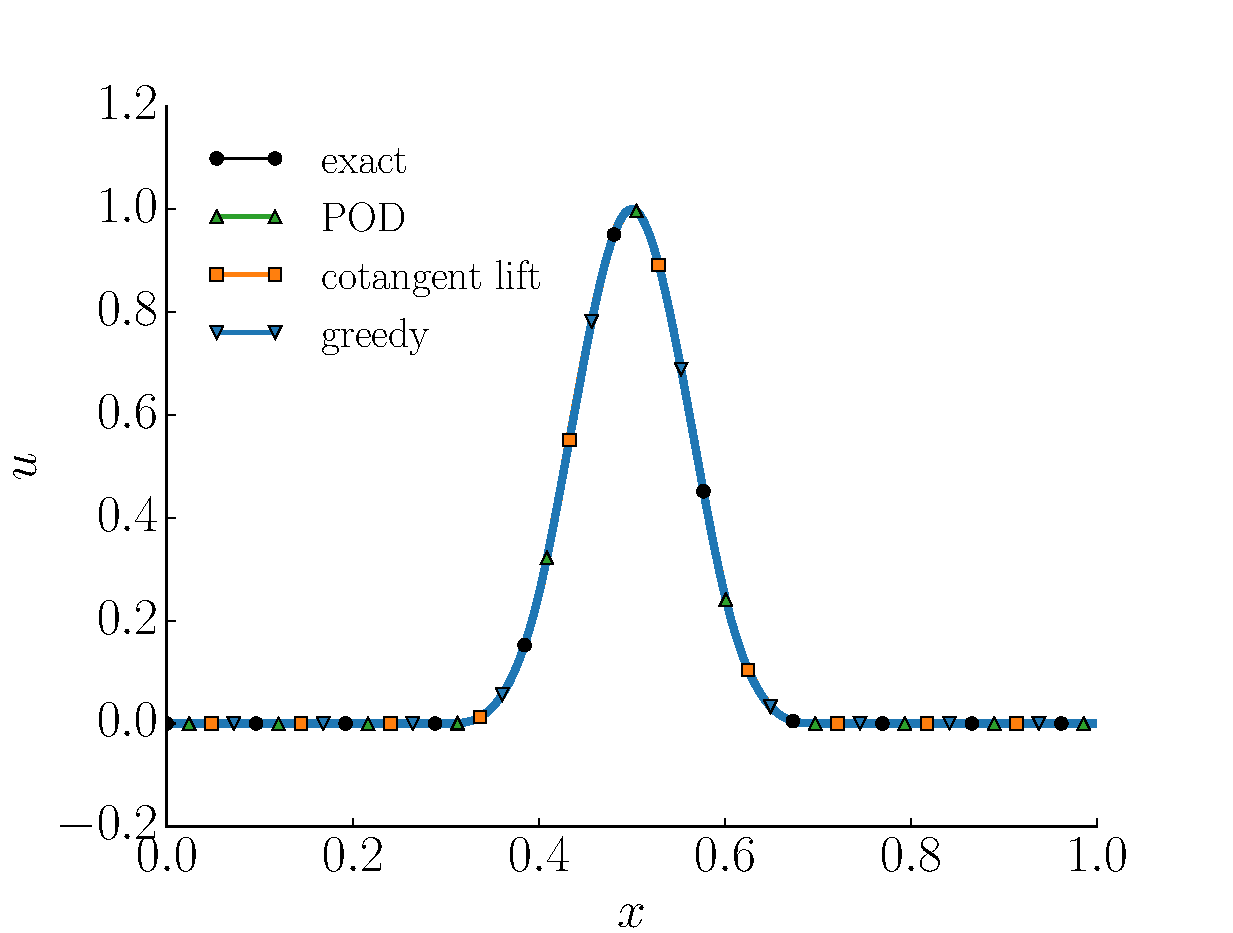
\includegraphics[width=0.4\textwidth]{./figs/wave/solution/solution_t0} &
%	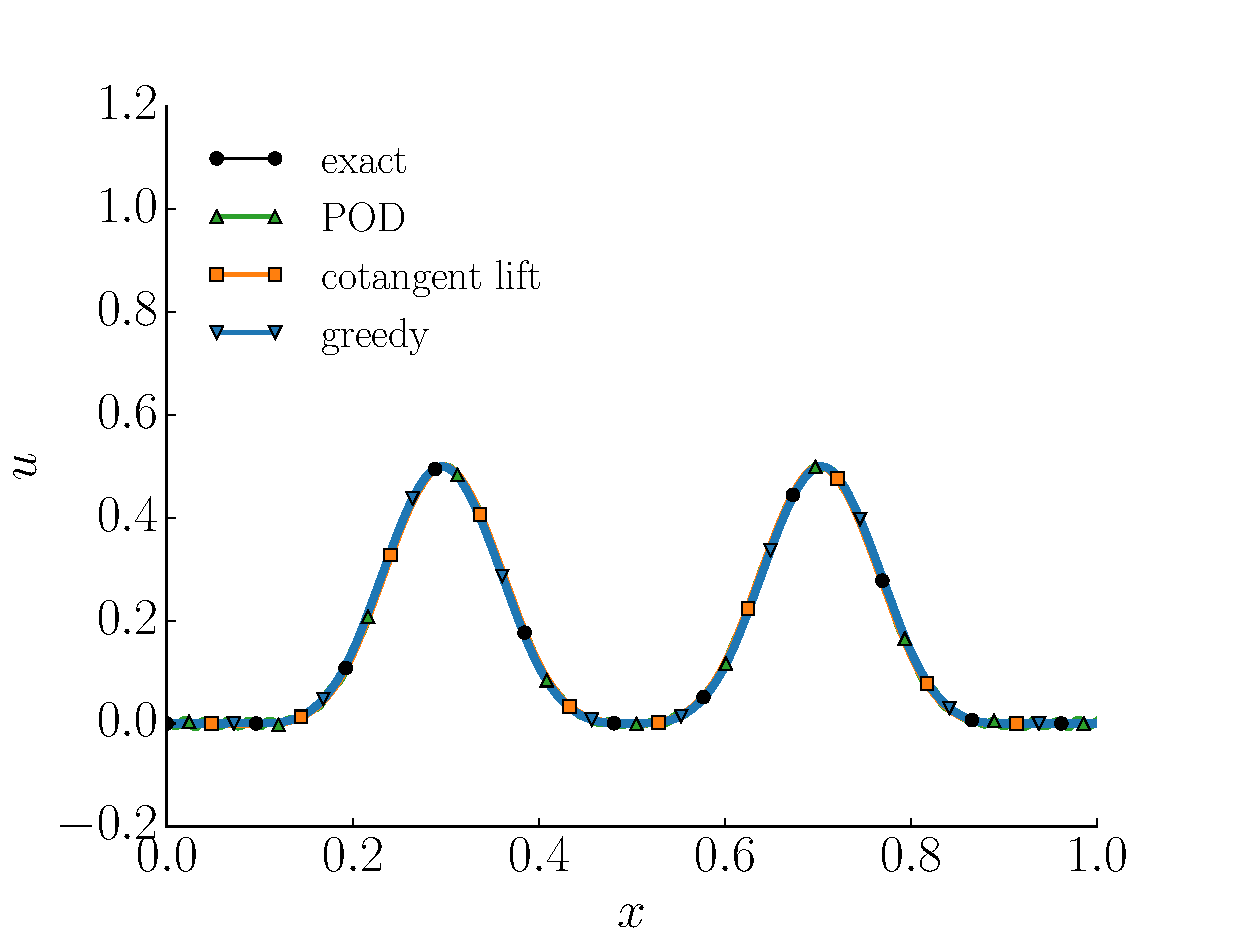
\includegraphics[width=0.4\textwidth]{./figs/wave/solution/solution_t1} \\
%	$t=0$ & $t = 1$
%\end{tabular}
%\end{center}
%\end{figure*}

%\begin{figure}[t]
%\centering
%\begin{tabular}{cc}
%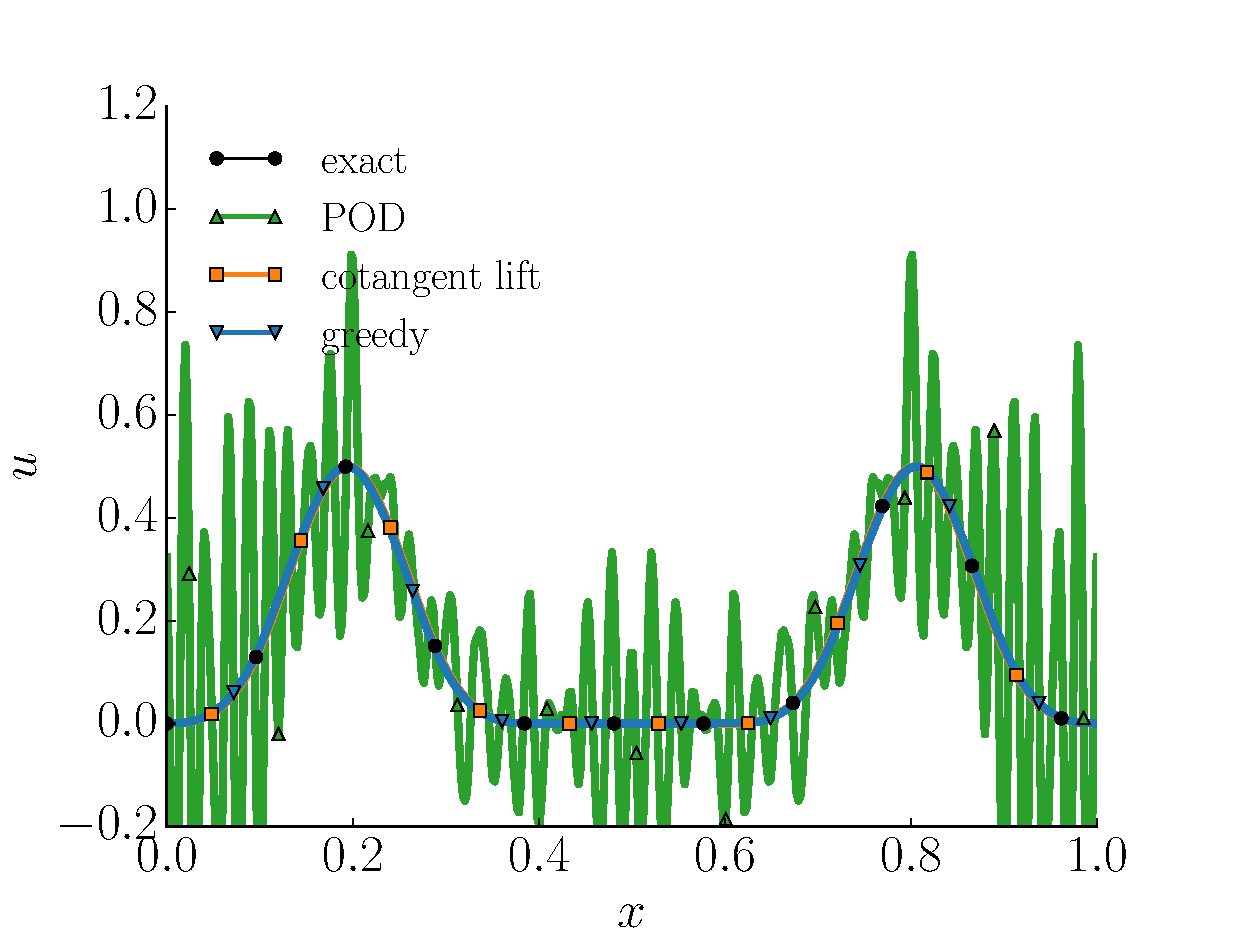
\includegraphics[width=0.4\textwidth]{./figs/wave/solution/solution_t2} \\
%	$t=2$
%\end{tabular}
%\caption{The solution $q$ at $t=0$, $t=1$ and $t=2$ of the linear wave equation for parameter value $c= 0.1019$ different from training parameters. Here the solution of full system together with the solution of the POD, cotangent lift, complex SVD and the greedy reduced system is presented.}\label{fig:NuRe:3}
%\end{figure}



%\begin{figure*}[t]
%\begin{center}
%\begin{tabular}{cc}
%	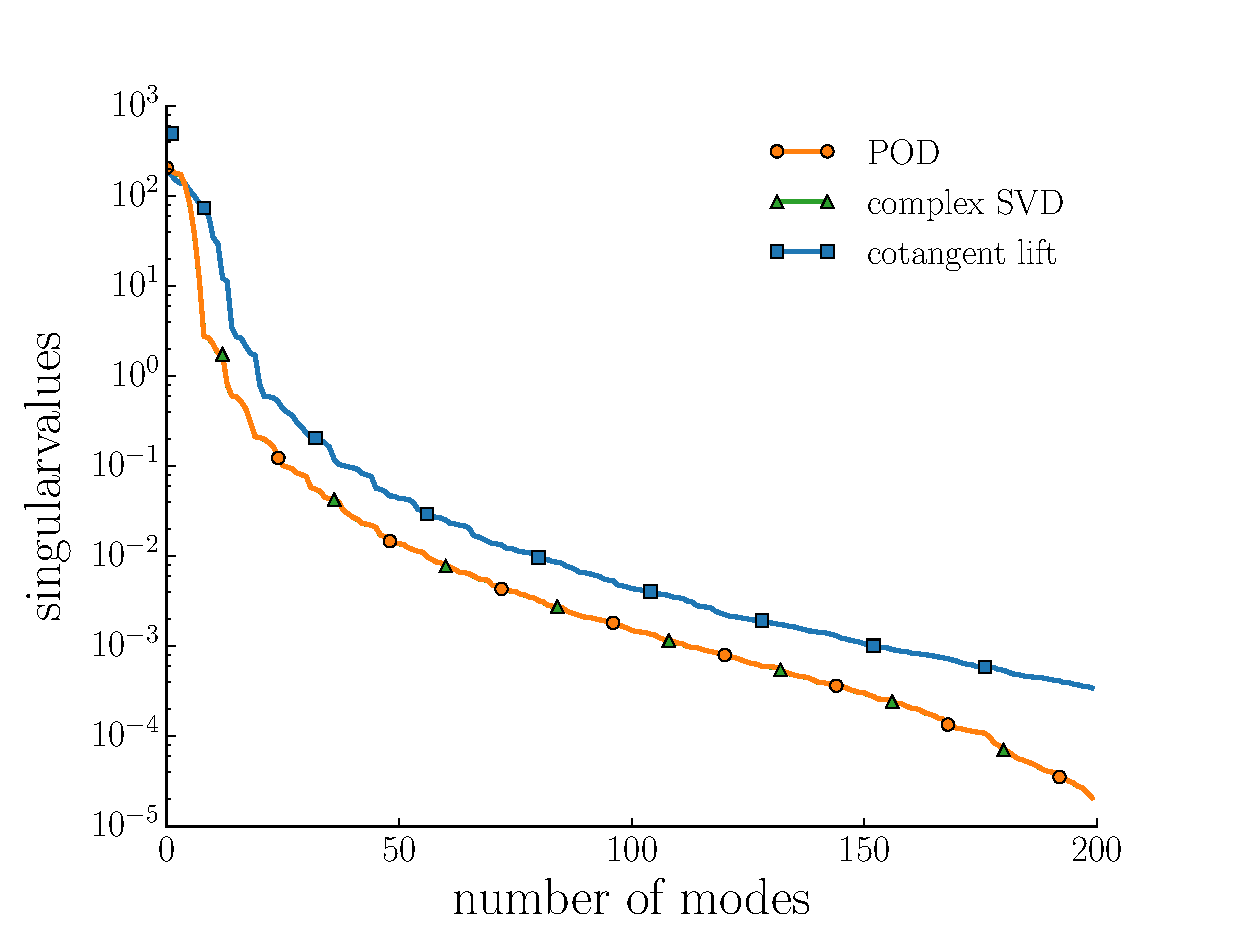
\includegraphics[width=0.5\textwidth]{./figs/wave/singular} &
%	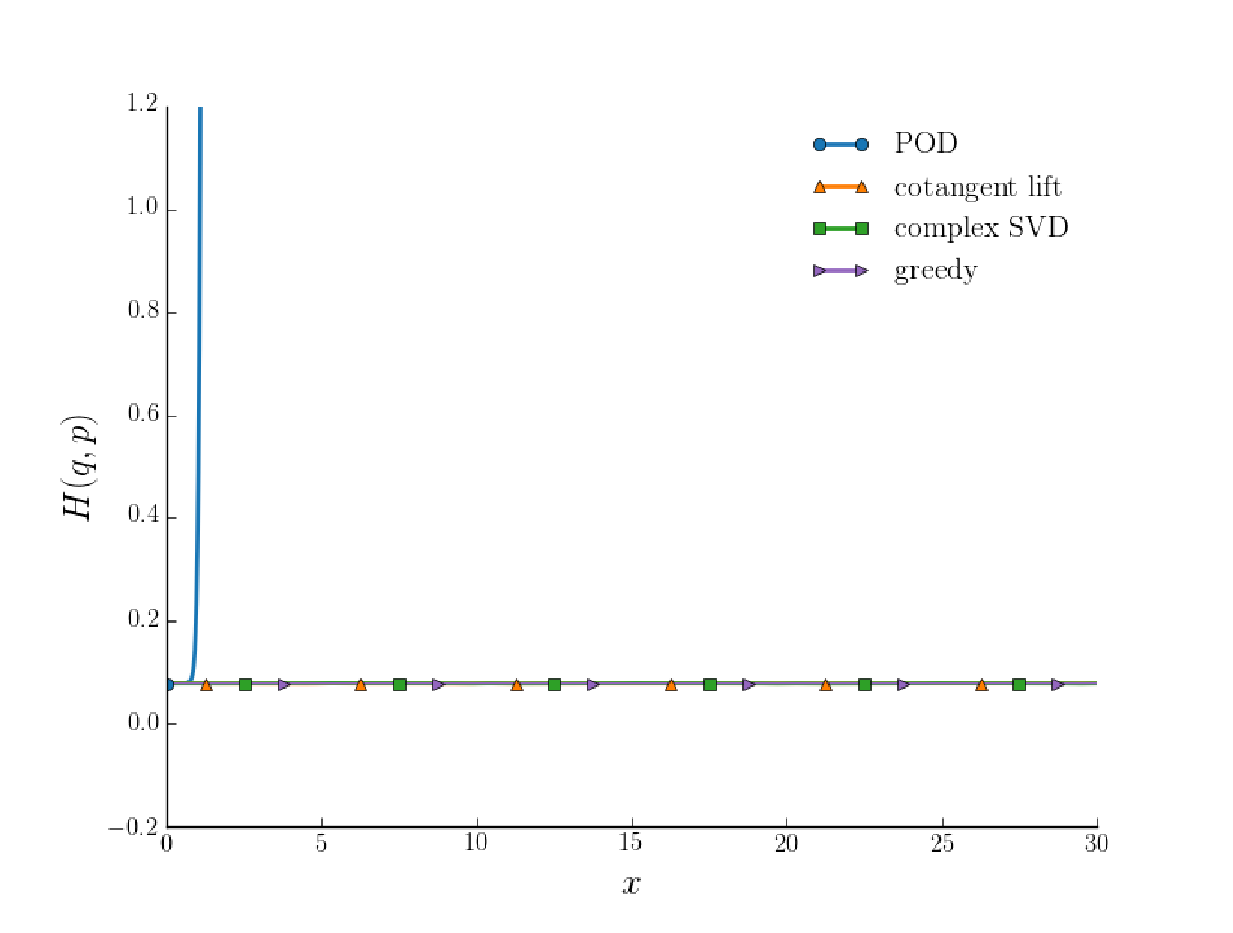
\includegraphics[width=0.5\textwidth]{./figs/wave/hamiltonian} \\
%	(a) & (b)
%\end{tabular}
%\end{center}
%\end{figure*}

%\begin{figure}[t] 
%\begin{center}
%\begin{tabular}{c}
%	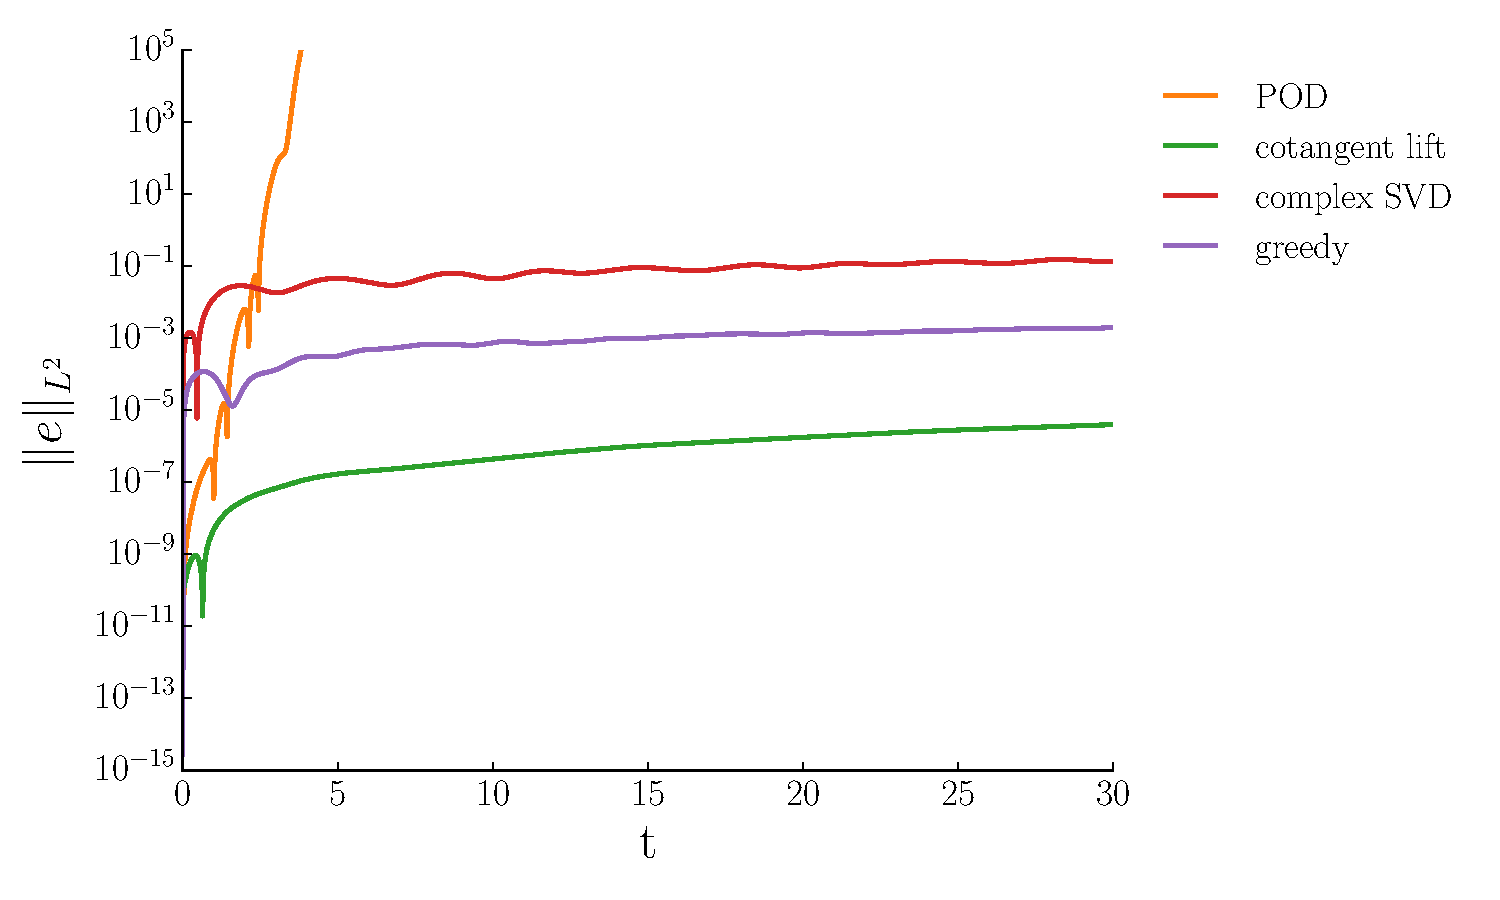
\includegraphics[width=0.5\textwidth]{./figs/wave/error} \\
%	(c)
%\end{tabular}
%\end{center}
%\caption{(a) The decay of singular values for POD, cotangent lift and complex SVD methods. (b) The $L^2$ error between the solution of th full system and the reduced system for different model reduction methods for $t \in [0,30]$. (c) Plot of the Hamiltonian function for $t \in [0,30]$.}\label{fig:NuRe:4}
%\end{figure}


%\begin{figure*}[t]
%  \centering
%  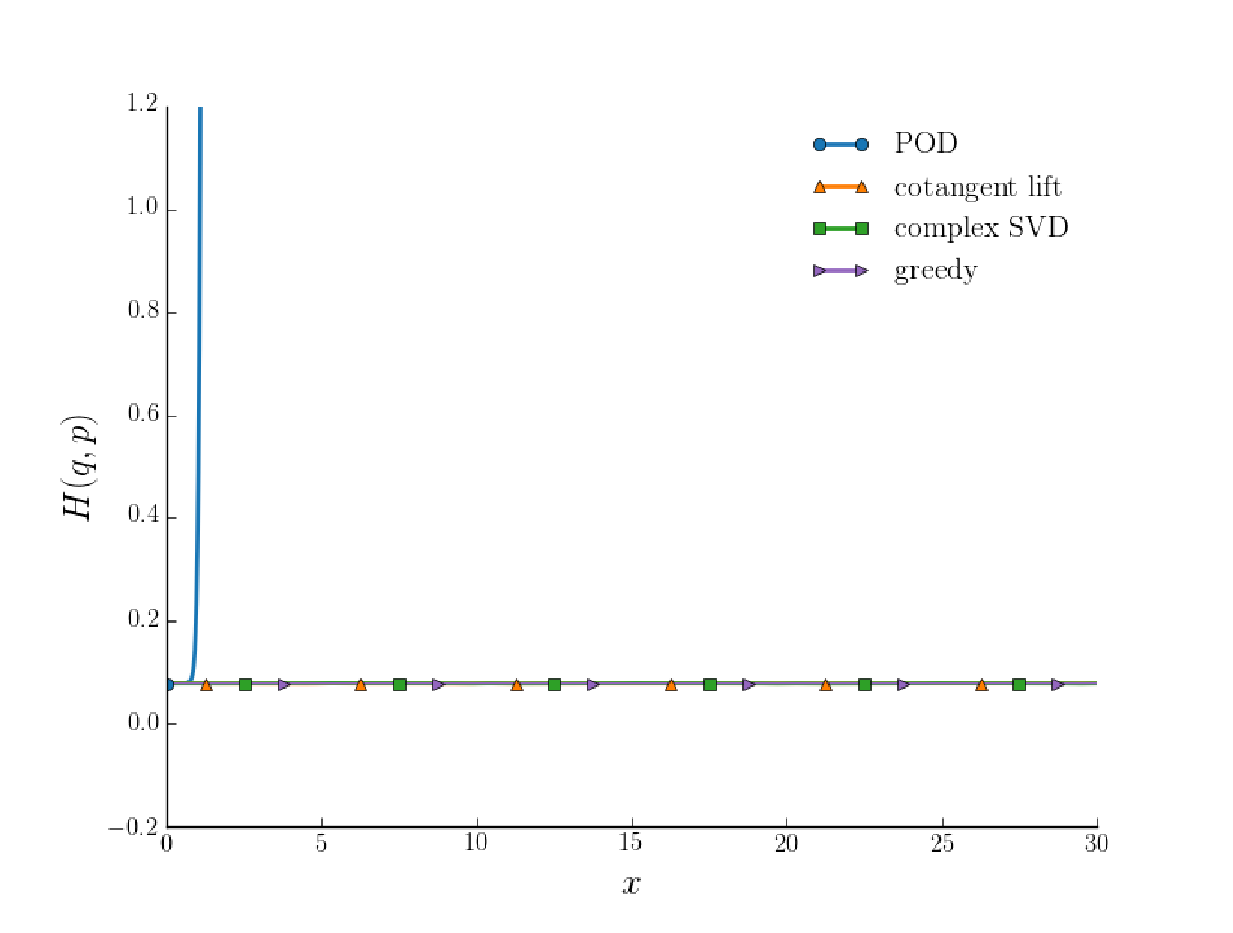
\includegraphics[width=0.5\textwidth]{./figs/wave/hamiltonian}
%  \label{fig:testfig}
%\end{figure*}

\begin{figure}

\begin{minipage}{.5\linewidth}
\centering
\subfloat[$t=0$]{\label{fig:NuRe:1a}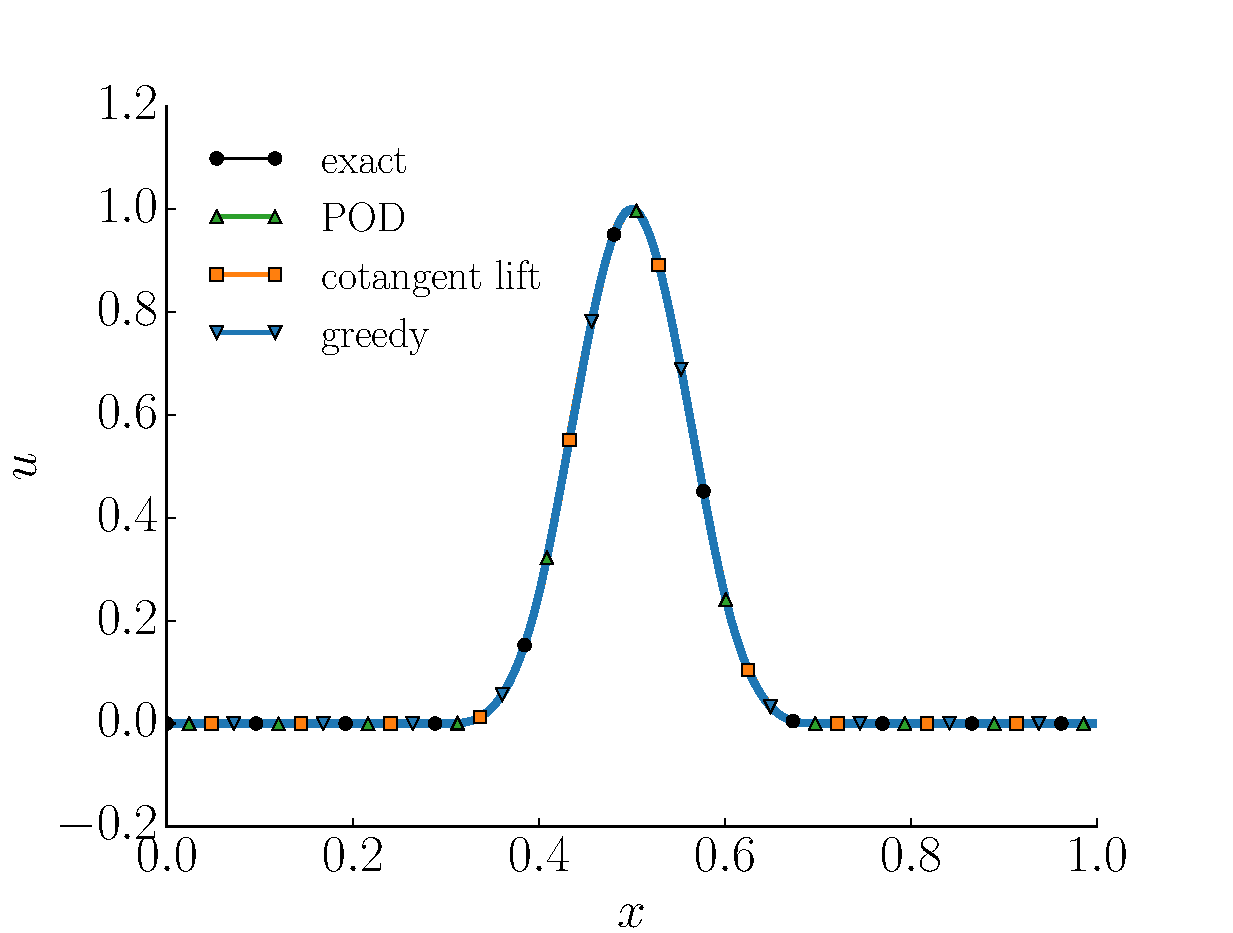
\includegraphics[width=1\textwidth]{./figs/wave/solution/solution_t0}}
\end{minipage}%
\begin{minipage}{.5\linewidth}
\centering
\subfloat[$t=1$]{\label{fig:NuRe:1b}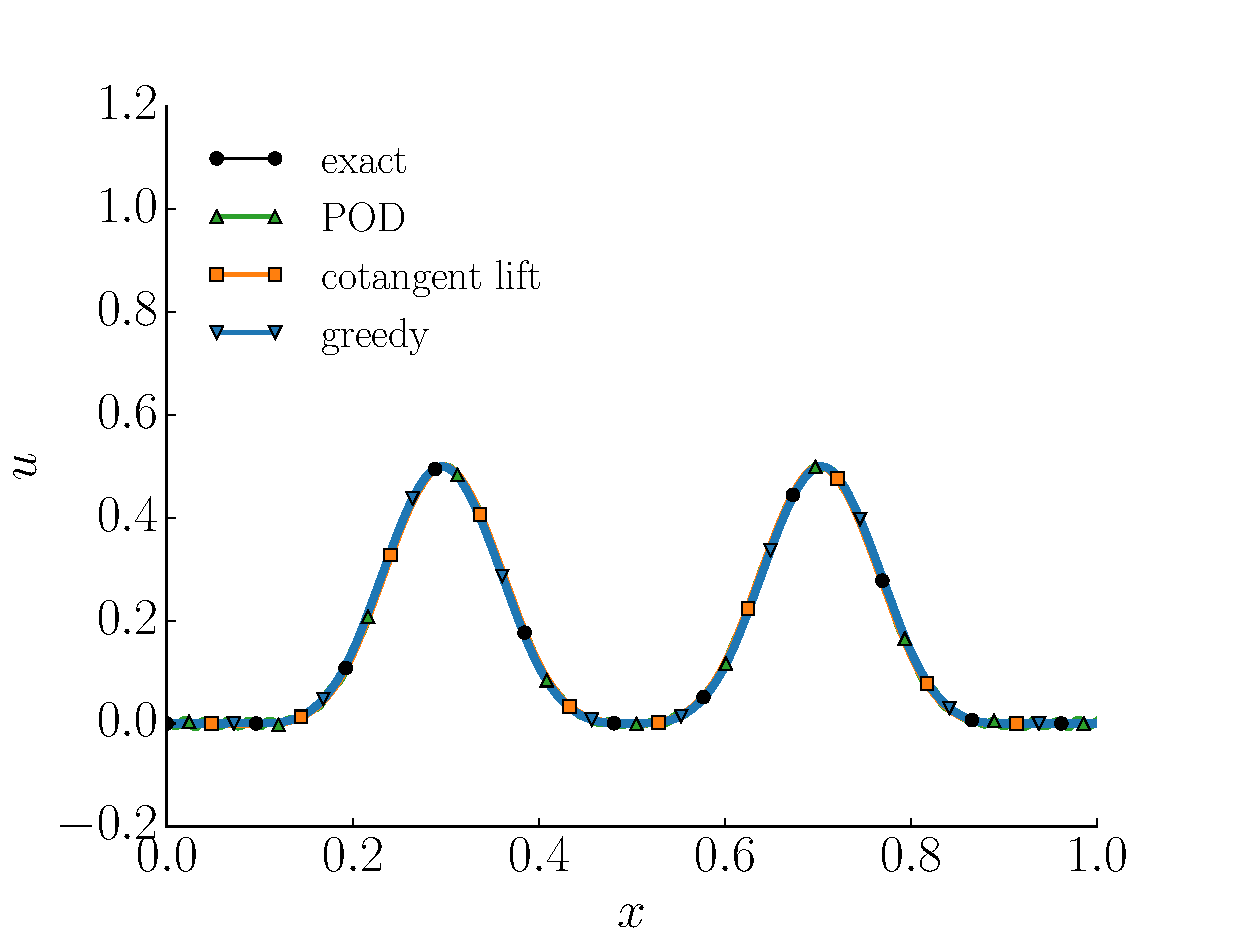
\includegraphics[width=\textwidth]{./figs/wave/solution/solution_t1}}
\end{minipage}\par\medskip
\centering
\subfloat[$t=2$]{\label{fig:NuRe:1c}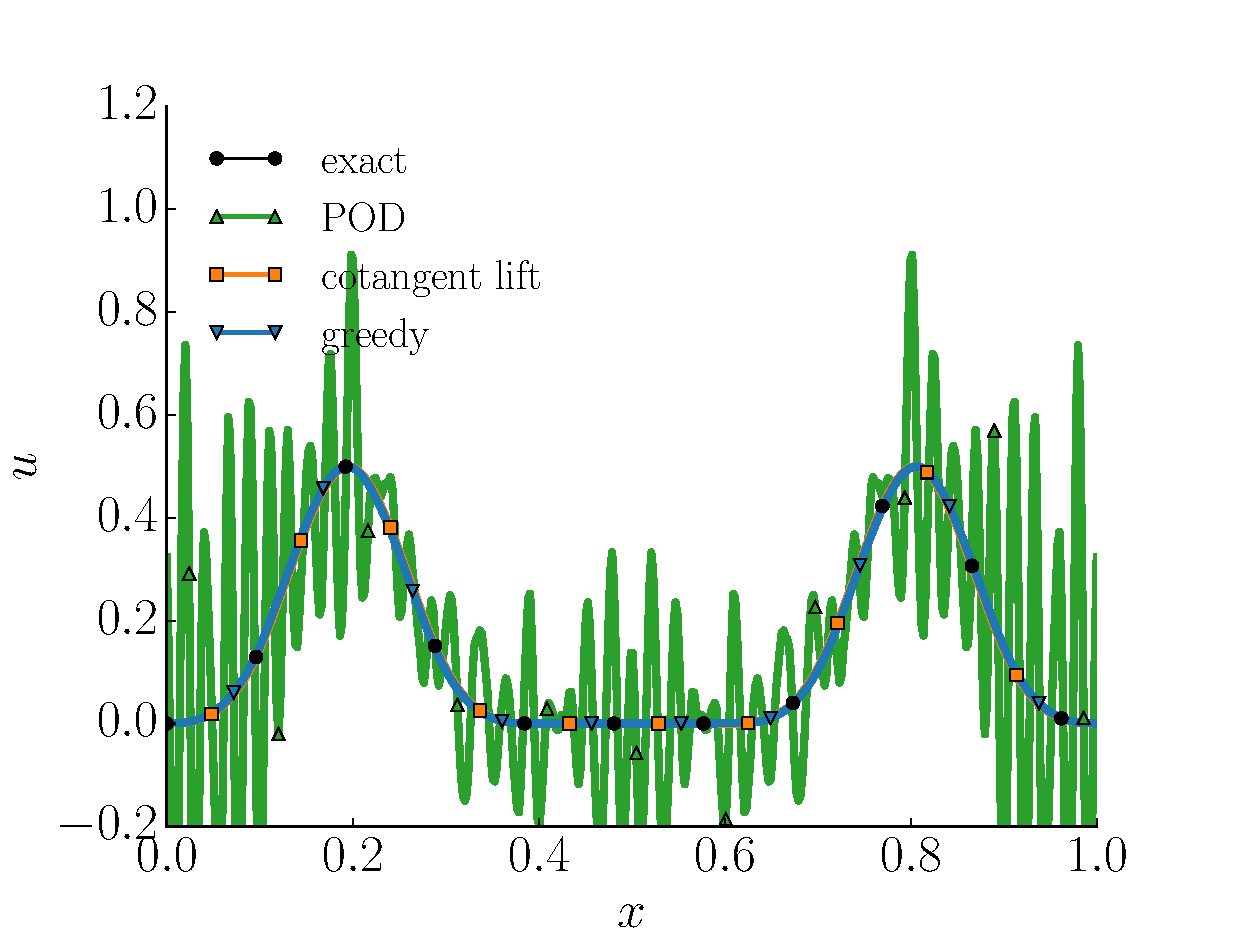
\includegraphics[width=0.5\textwidth]{./figs/wave/solution/solution_t2}}
\caption{The solution $q$ at $t=0$, $t=1$ and $t=2$ of the linear wave equation for parameter value $c= 0.1019$ different from training parameters. Here the solution of full system together with the solution of the POD, cotangent lift, complex SVD and the greedy reduced system is presented.}
\label{fig:NuRe:1}
\end{figure}

\begin{figure}

\begin{minipage}{.5\linewidth}
\centering
\subfloat[]{\label{fig:NuRe:2c}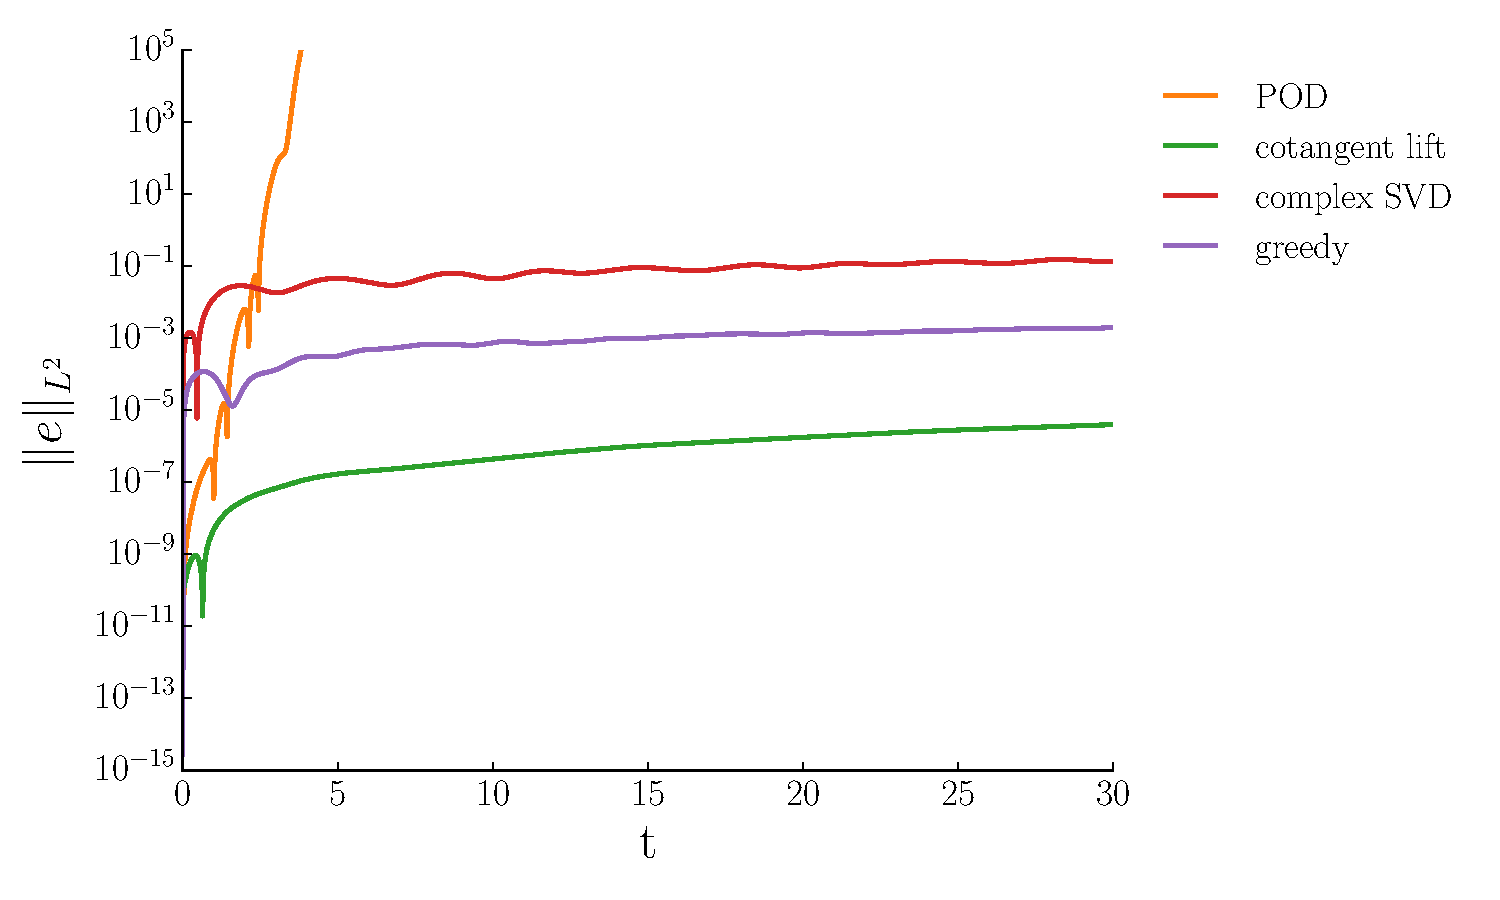
\includegraphics[width=\textwidth]{./figs/wave/error}}
\end{minipage}%
\begin{minipage}{.5\linewidth}
\centering
\subfloat[]{\label{fig:NuRe:2b}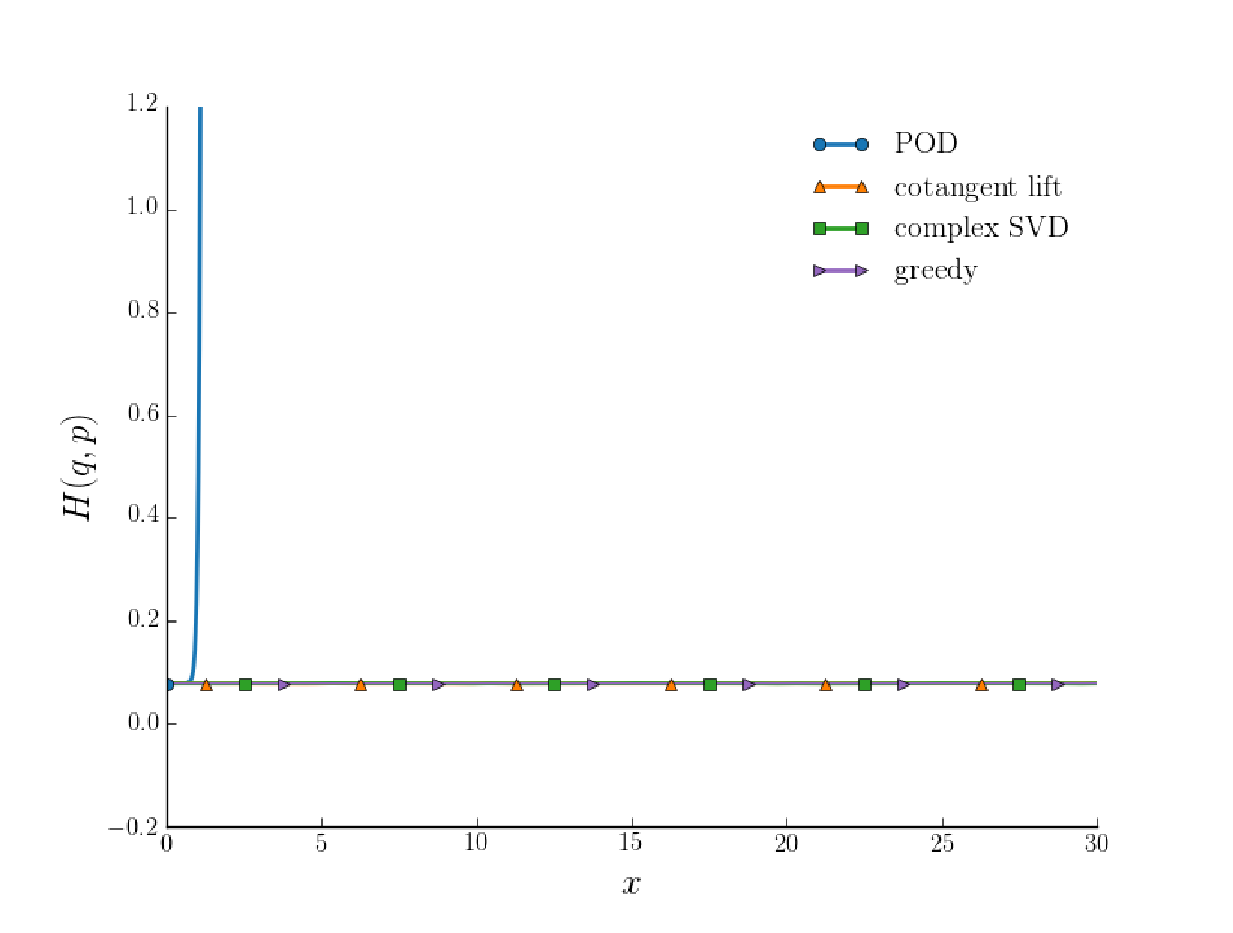
\includegraphics[width=\textwidth]{./figs/wave/hamiltonian}}
\end{minipage}\par\medskip
\centering
%\subfloat[]{\label{fig:NuRe:2c}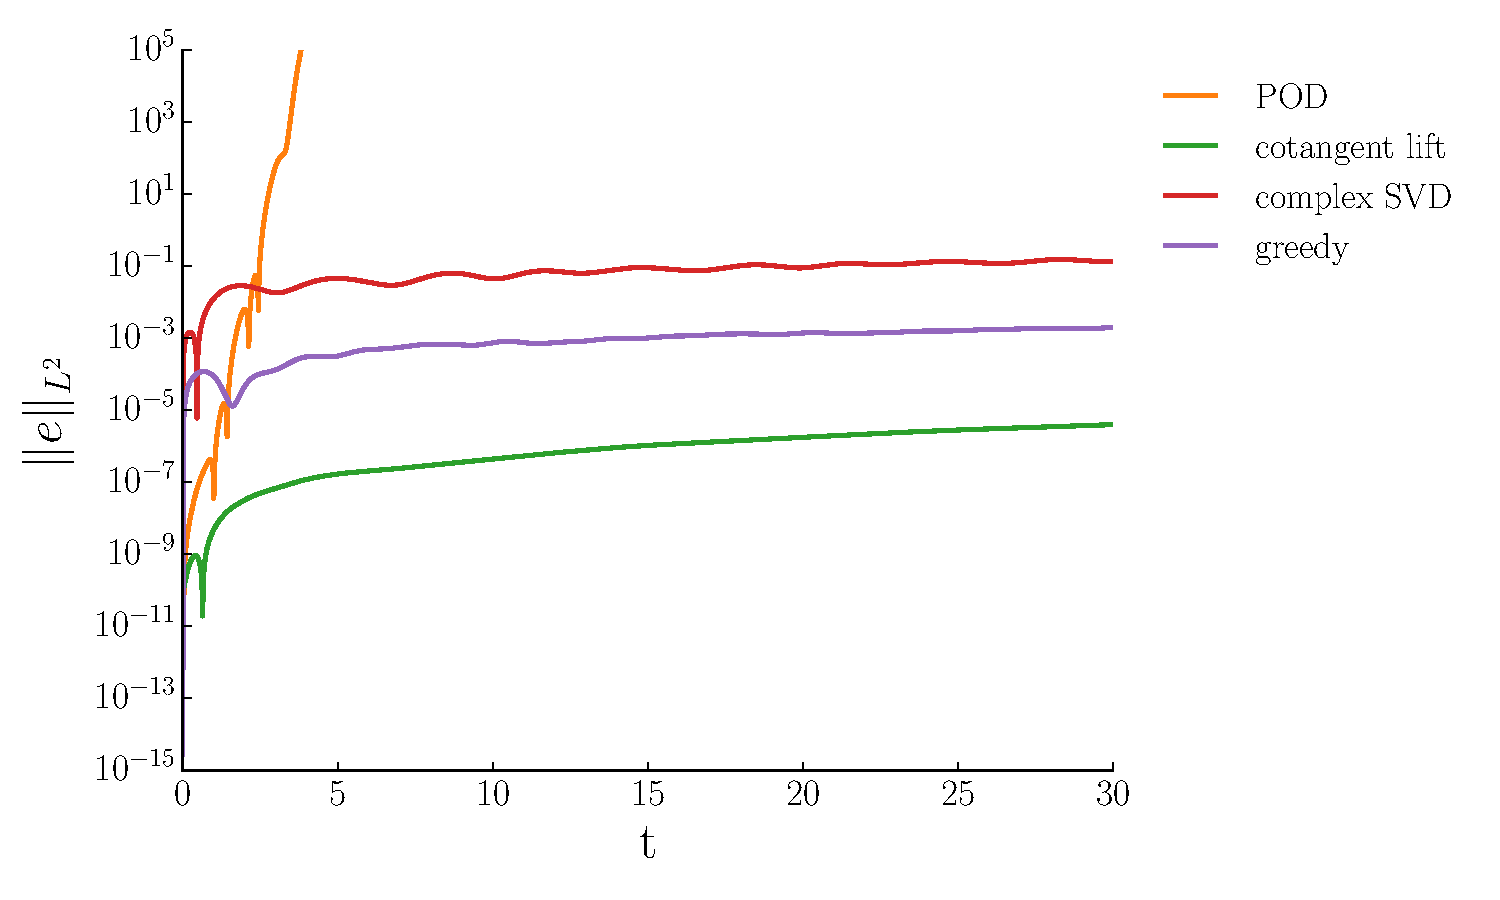
\includegraphics[width=0.5\textwidth]{./figs/wave/error}}

\caption{(a) The decay of singular values for POD, cotangent lift and complex SVD methods. (b) Plot of the Hamiltonian function for $t \in [0,30]$. (c) The $L^2$ error between the solution of the full system and the reduced system for different model reduction methods for $t \in [0,30]$.}
\label{fig:NuRe:2}
\end{figure}


\subsection{Nonlinear Schr\"odinger equation} Let us consider the one-dimensional parametric Schr\"odinger equation
\begin{equation} \label{eq:NuRe:10}
\left\{
\begin{aligned}
	& i u_t(t,x,\epsilon) = - u_{xx}(t,x,\epsilon) - \epsilon |u(t,x,\epsilon)|^2 u(t,x,\epsilon),\\
	& u(0,x) = u_0(x),
\end{aligned}
\right.
\end{equation}
where $u$ is a complex valued wave function, $i$ is the imaginary unit, $|\cdot|$ is the modulus operator and $\epsilon$ is a parameter that belongs to the interval $\Gamma = [0.9,1.1]$. We consider periodic boundary conditions, i.e., $x$ belongs to a one dimensional torus of length $L$. We consider the initial condition
\begin{equation} \label{eq:NuRe:11}
	u_0(x) = \frac{\sqrt 2}{\cosh(x - x_0)} \exp(i\frac{c(x-x0)}{2}),
\end{equation}
for a positive constant $c$. In quantum mechanics, the quantity $|u(t,x)|^2$ represents the probability of finding the system in state $x$ at time $t$. For the choice of $\epsilon = 1$, $|u(x,t)|$ becomes a solitary wave, and the initial condition will be transported in the positive $x$ direction with a constant speed. For other choices of $\epsilon$, the solution comprises an ensemble of solitary waves, moving in either direction \cite{Faou:2012vh}. 

By introducing the real and imaginary variables $u = p + iq$, we can rewrite (\ref{eq:NuRe:10}) in canonical form as
\begin{equation} \label{eq:NuRe:12}
\left\{
\begin{aligned}
 q_t &= p_{xx} + \epsilon (q^2+p^2)p, \\
 p_t &= -q_{xx} - \epsilon (q^2 + p^2)q,
\end{aligned}
\right.
\end{equation}
with the Hamiltonian function
\begin{equation} \label{eq:NuRe:13}
	H(q,p) = \int_{0}^{L} (q_x^2 + p_x^2) + \frac \epsilon 2 (q^2 + p^2)^2\ dx.
\end{equation}

We discretize the torus into $N$ equidistant points and take $\Delta x = L/N$, $x_i = i\Delta x$, $q_i=q(t,x_i,\epsilon)$ and $p_i = p(t,x_i,\omega)$ for $i = 1 ,\dots,N$. A central finite differences scheme is used to discretize (\ref{eq:NuRe:12}) as
\begin{equation}  \label{eq:NuRe:14}
	\frac{d}{dt} \mathbf z = \mathbb J_{2N} L\mathbf z + \mathbb J_{2N} \mathbf g(\mathbf z).
\end{equation}
Here $\mathbf z = (q_1,\dots,q_N,p_1,\dots,p_n)^T$ and
\begin{equation}  \label{eq:NuRe:15}
	L = 
	\begin{pmatrix}
		D_{xx} & 0_N \\
		0_N & D_{xx}
	\end{pmatrix}
\end{equation}
with $D_{xx}$ being the central finite differences matrix operator for periodic boundary conditions. $\mathbf g$ is a vector valued nonlinear function defined as
\begin{equation}  \label{eq:NuRe:16}
	\mathbf g(\mathbf z) =
	\begin{pmatrix}
	(q_1^2 + p_1^2)q_1 \\
	\vdots \\
	(q_N^2 + p_N^2)q_N \\
	(q_1^2 + p_1^2)p_1 \\
	\vdots \\
	(q_N^2 + p_N^2)p_N
	\end{pmatrix}.
\end{equation}
We discretize the Hamiltonian to obtain
\begin{equation}  \label{eq:NuRe:17}
	H_{\Delta x}(\mathbf z) = {\Delta x}\sum_{i=1}^{N} \left( \frac{q_i q_{i-1} - q_i^2}{\Delta x ^2} + \frac{p_i p_{i-1} - p_i^2}{\Delta x ^2} + \frac \epsilon 4 (p_i^2 + q_i^2)^2  \right).
\end{equation}
We use a Str\"omer-Verlet (\ref{eq:Hasy:13}) scheme for time integration. Since the Hamiltonian function (\ref{eq:NuRe:17}) is non-separable, this scheme becomes implicit so in each time iteration, a system of nonlinear equations is solved using Newton's iteration. We summarize the physical and numerical parameters for the full model in the following table

\vspace{0.5cm}
\begin{center}
\begin{tabular}{|l|l|}
\hline
Domain length & $L = 2\pi /l$ \\
Domain scaling factor & $l = 0.11$ \\
wave speed & $c =1$\\
No. grid points & $N = 256$ \\
Space discretization size & $\Delta x = 0.2231$ \\
Time discretization size & $\Delta t = 0.01$ \\
\hline
\end{tabular}
\end{center}
\vspace{0.5cm}

Regarding computation of the nonlinear terms of reduced systems, {\edit we} compare the DEIM with the symplectic DEIM. For generation of the DEIM reduced basis we apply Algorithm \ref{alg:MoOr:1} to the set of nonlinear snapshots. Algorithm \ref{alg:SyMo:4} is used to construct a reduced basis appropriate for the symplectic DEIM. As input, we provide the symplectic basis generated by Algorithm \ref{alg:SyMo:3} with the set of nonlinear snapshots and a tolerance for the error $\delta = 10^{-4}$.

We compared the reduced system obtained by the greedy algorithm with the cotangent lift, complex SVD, DEIM, symplectic DEIM and also POD. For the SVD-based methods, we discretize the parameter space $[0.9,1.1]$ into $M=500$ equidistant grid points to recover the discrete parameter space $\Gamma_M = \{\epsilon_1,\dots,\epsilon_M \}$, and gather trajectory snapshots for each $\epsilon_i$ for $i = 1,\dots,M$ in the snapshots matrix $S$. All reduced system are taken to have identical sizes ($k=90$ for symplectic methods and $k=180$ for the POD method). Following algorithm \ref{alg:SyMo:3} we construct the reduced system using the same discrete parameter space $\Gamma_M$. The tolerance for the error in the Hamiltonian is set to $\delta = 10^{-3}$. Moreover, for DEIM and symplectic DEIM, we construct bases of size $k'=80$. Note that in the reduced system, generated in the symplectic DEIM, will be of size $k+k'=170$.

The cost of the offline stage is reduced to 20\% when using the greedy method for constructing a symplectic basis of size $k=90$, as compared to the SVD-based methods. The online stage, i.e., time integration for a new parameter in $\Gamma$, is generally more than 3 times faster than the original system. We point out that the efficiency of reduced systems are implementation and platform dependent.

%The duration of the online and offline stages for different model reduction techniques are summarized in table below. The offline time for the cotangent lift and the complex SVD consist of time integration of the full model for all the parameters in the discrete parameter space $\Omega_M$. This is while the greedy method requires substantially shorter offline stage to construct a reduced basis of size $k = 90$. For a reduced system of size $k=90$, all methods almost have the same online duration. The efficiency of reduced systems compared to the full system are heavily implementation dependent, nevertheless solving the reduced systems with our implementation is more than 3 times faster than solving the original system.

%\vspace{0.5cm}
%\begin{center}
%\begin{tabular}{c|cc}
% & offline (hours) & online (seconds) \\
%\hline
%full system & - & 187 \\
%cotangent lift & 25.8 & 59$\pm 1$ \\
%complex SVD & 25.8 & 59$\pm 1$ \\
%greedy & 4.6 & 59$\pm 1$ \\
%greedy + SDEIM & 4.7 & ???
%\end{tabular}
%\end{center}
%\vspace{0.5cm}


%\begin{figure*}[t]
%\begin{center}
%\begin{tabular}{cc}
%	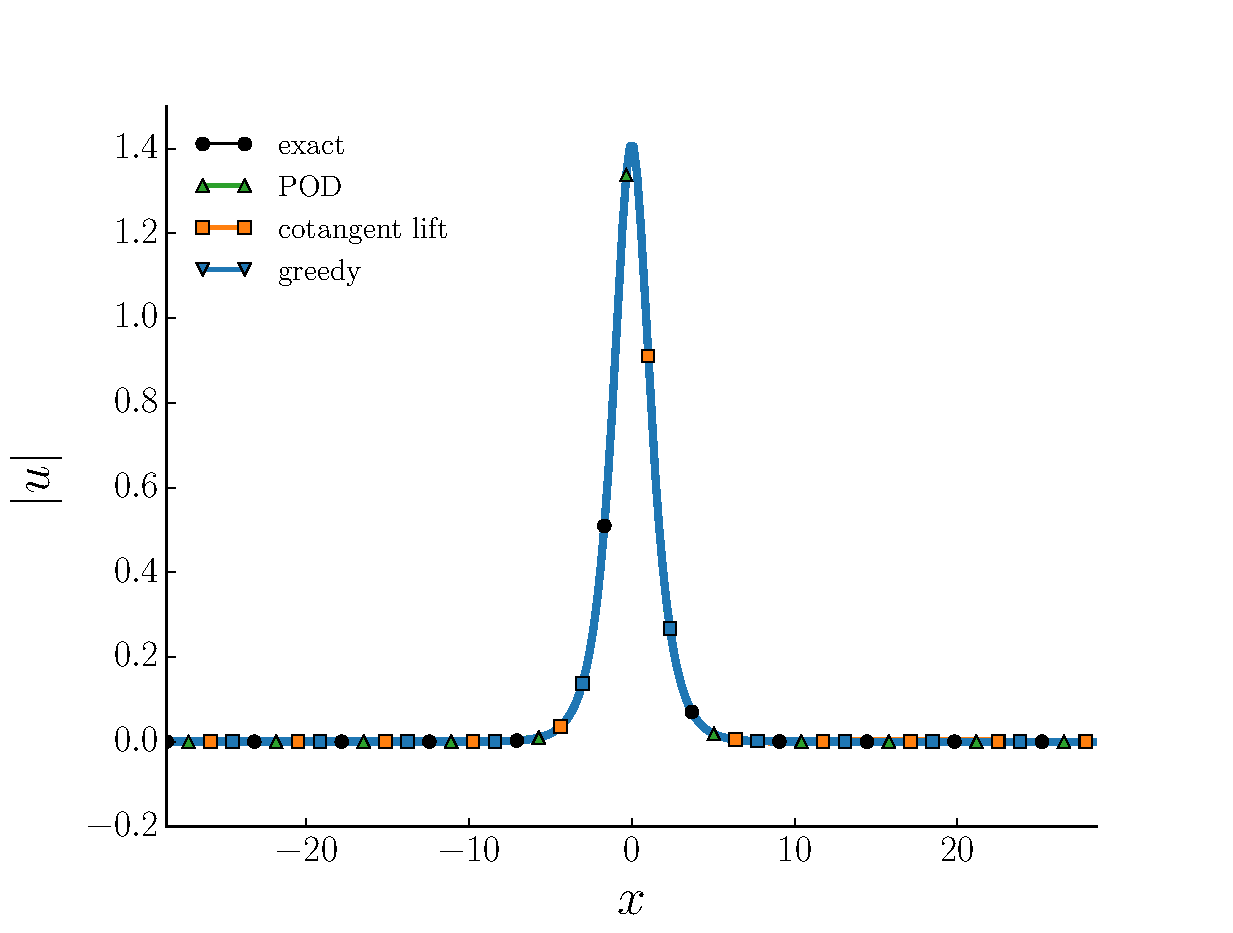
\includegraphics[width=0.5\textwidth]{./figs/schrodinger/solution/solution_t0} &
%	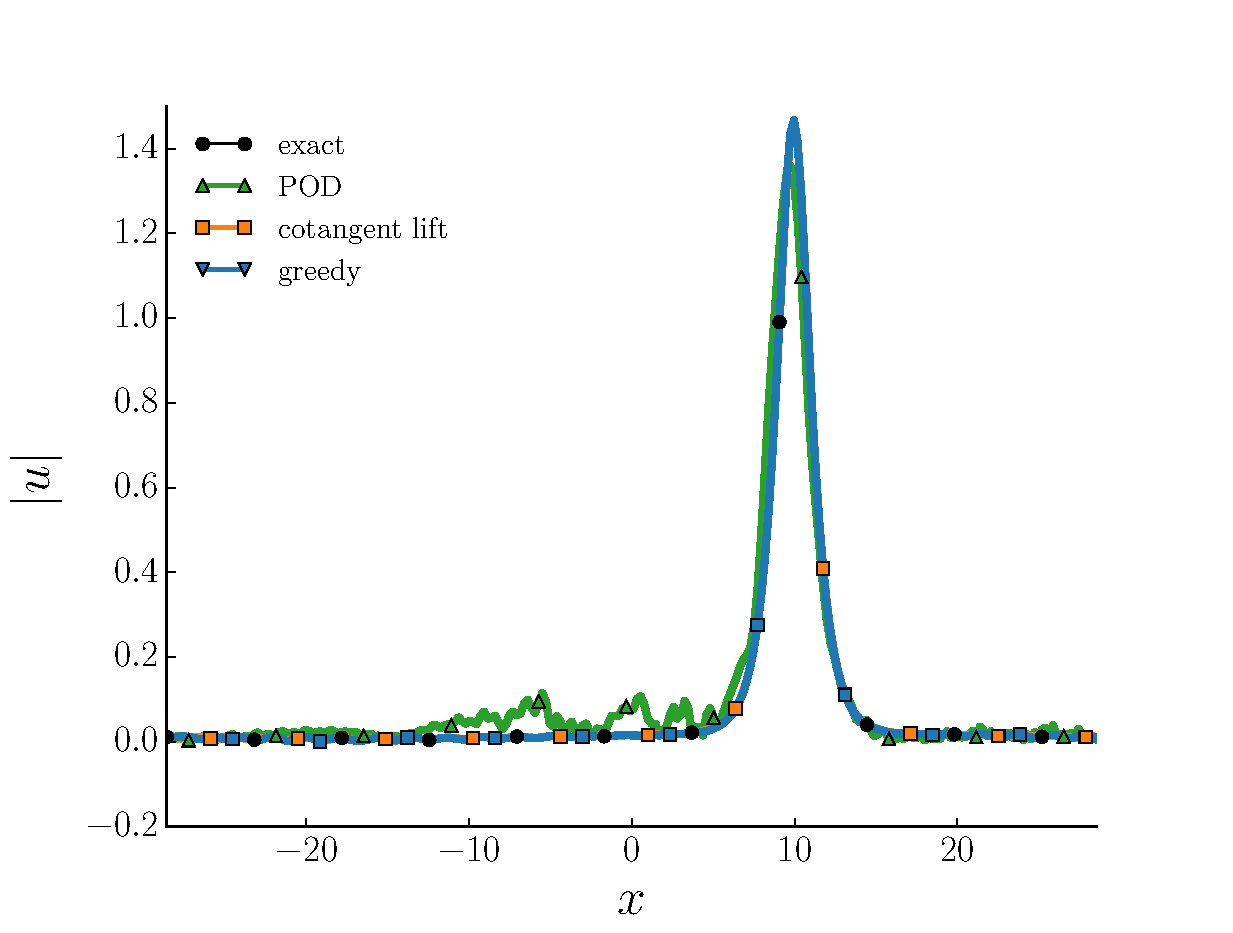
\includegraphics[width=0.5\textwidth]{./figs/schrodinger/solution/solution_t10} \\
%	$t = 0$ & $t = 10$
%\end{tabular}
%\end{center}
%\end{figure*}
%
%\begin{figure}[t] 
%\begin{center}
%\begin{tabular}{c}
%	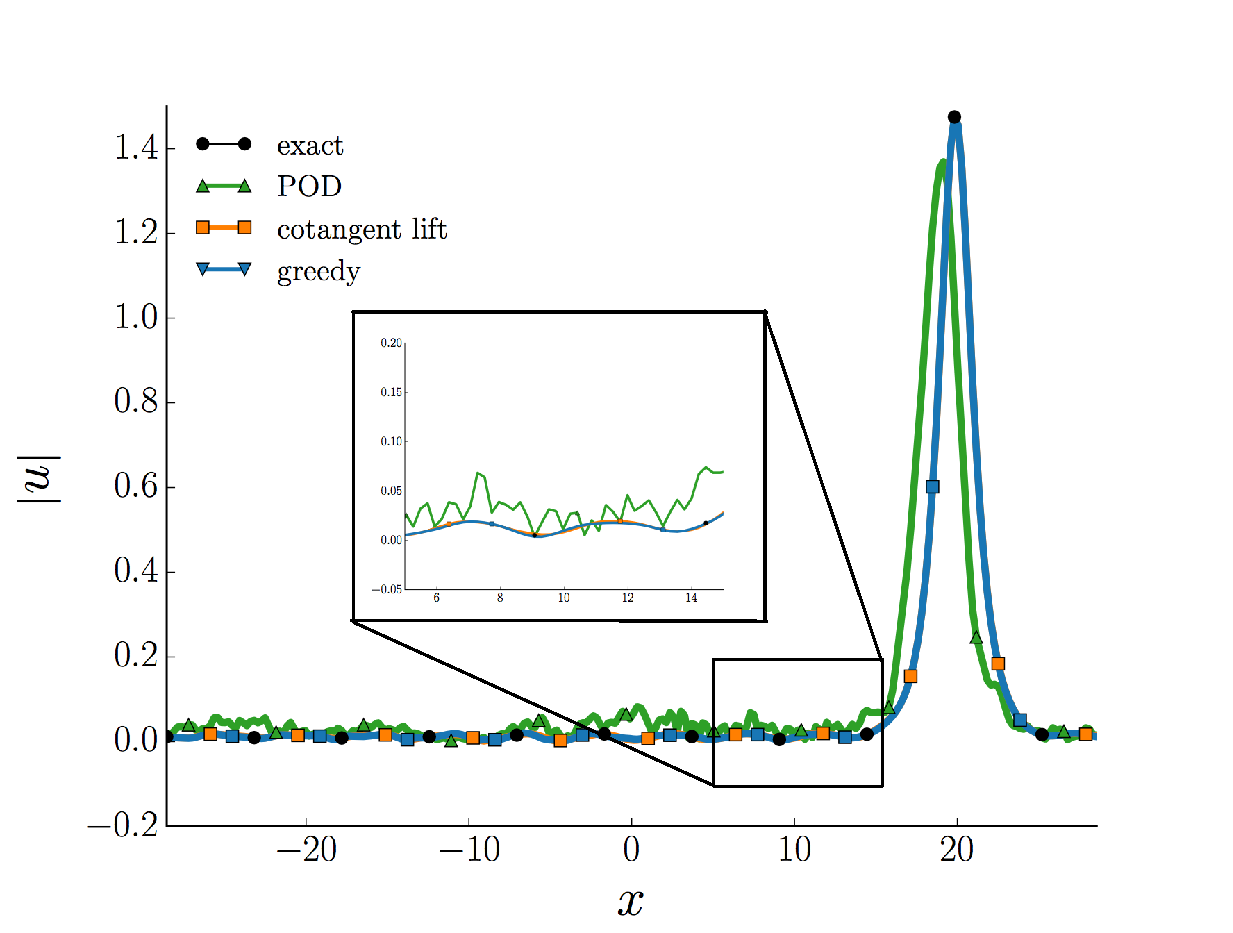
\includegraphics[width=0.5\textwidth]{./figs/schrodinger/solution/solution_t20}\\
%	$$t = 20$$
%\end{tabular}
%\end{center}
%\caption{The solution $|u(t,x)| = \sqrt{q^2 + p^2}$ at $t=0$, $t=10$ and $t=20$ of the Nonlinear Schr\"odinger equation for parameter value $\epsilon = 1.0932$. Here the solution of full system together with the solution of the POD, cotangent lift, complex SVD and the greedy reduced system is presented.}\label{fig:NuRe:1}
%\end{figure}
%
%\begin{figure*}[t]
%\begin{center}
%\begin{tabular}{cc}
%	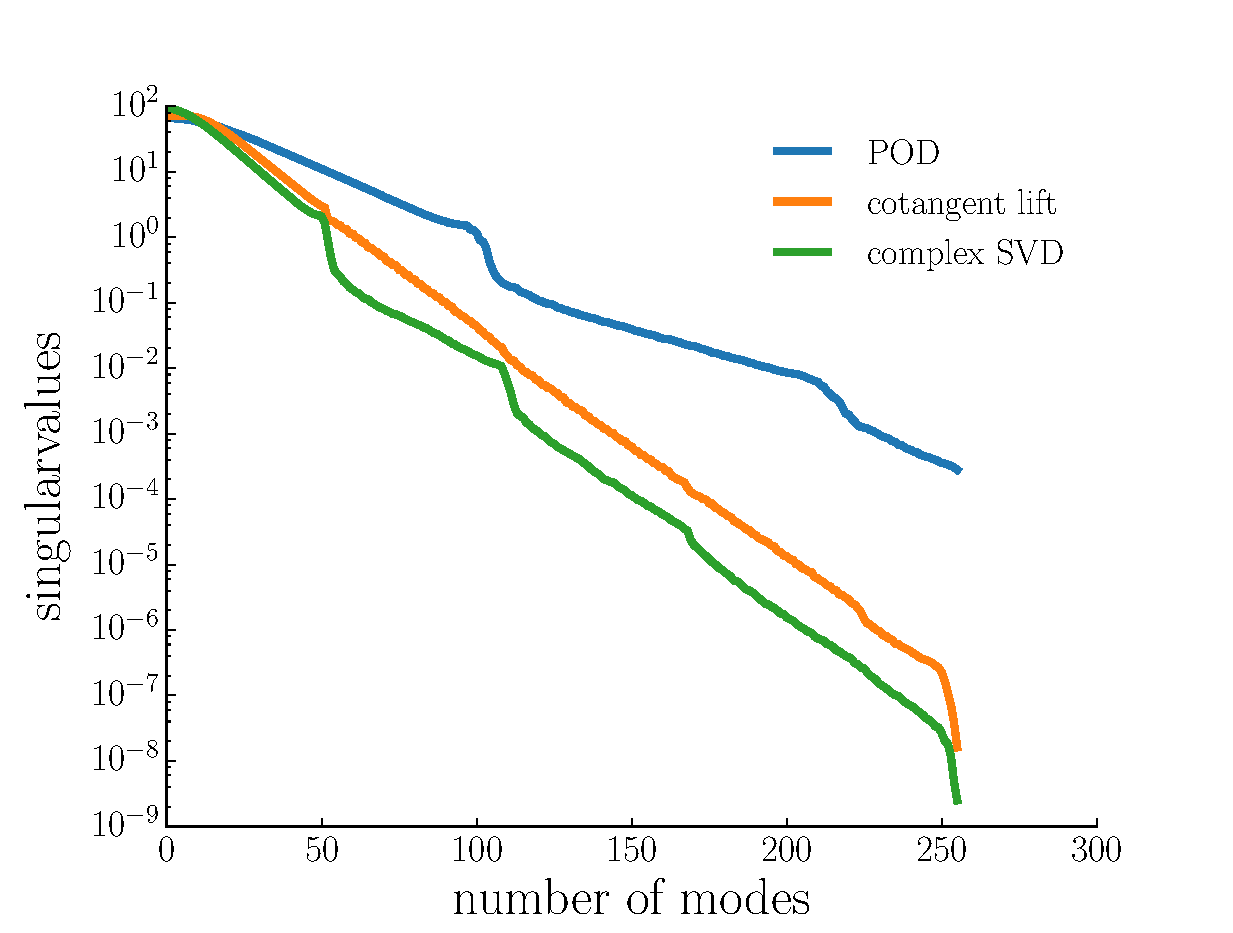
\includegraphics[width=0.5\textwidth]{./figs/schrodinger/singular} &
%	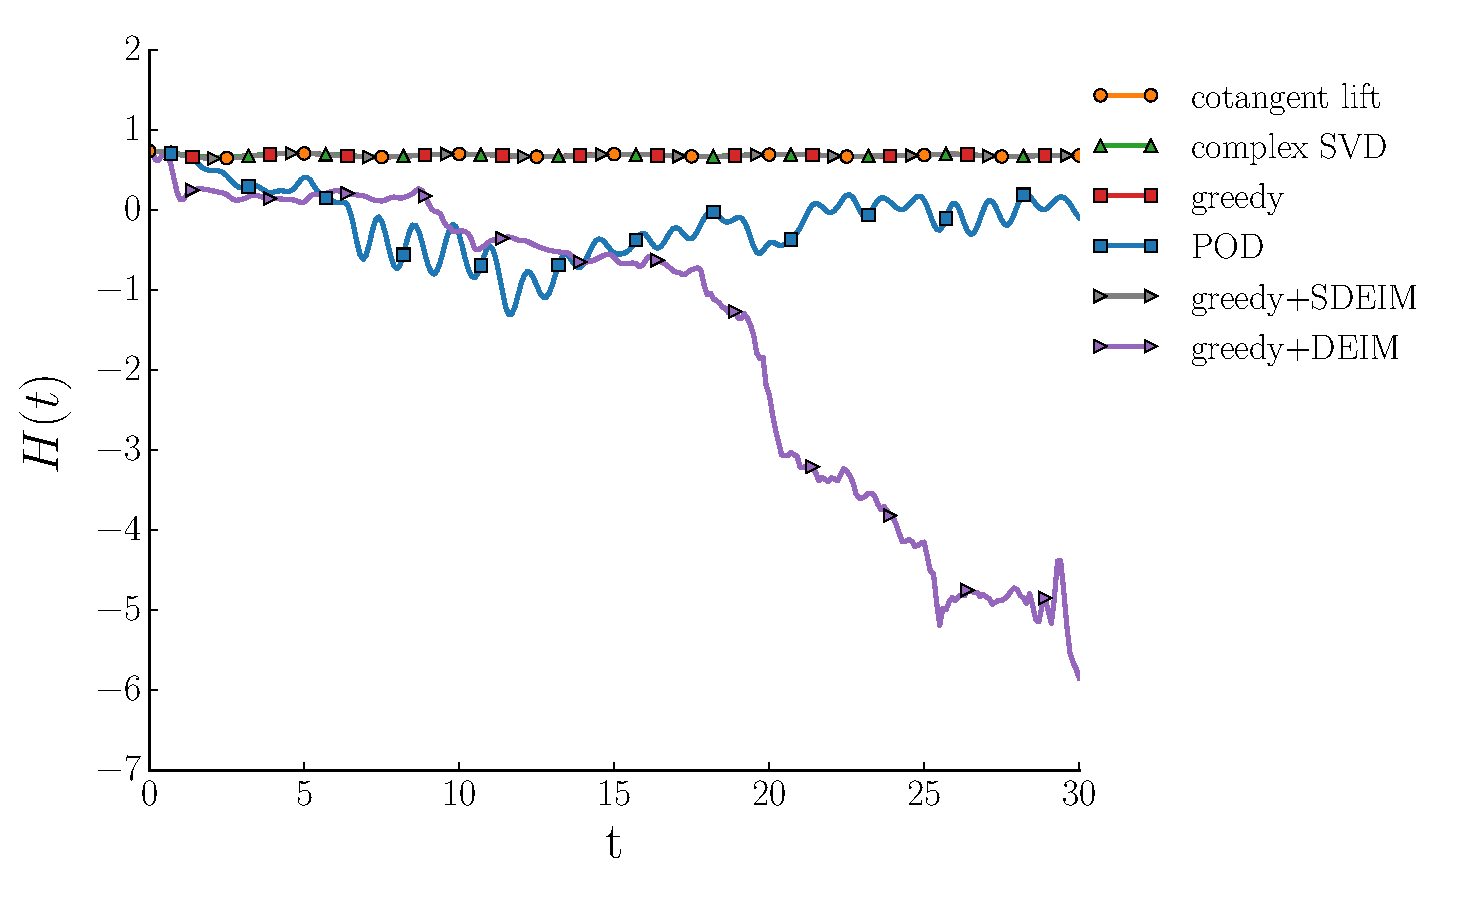
\includegraphics[width=0.5\textwidth]{./figs/schrodinger/hamiltonian} \\
%	(a) & (b)
%\end{tabular}
%\end{center}
%\end{figure*}
%
%\begin{figure}[t] 
%\begin{center}
%\begin{tabular}{c}
%	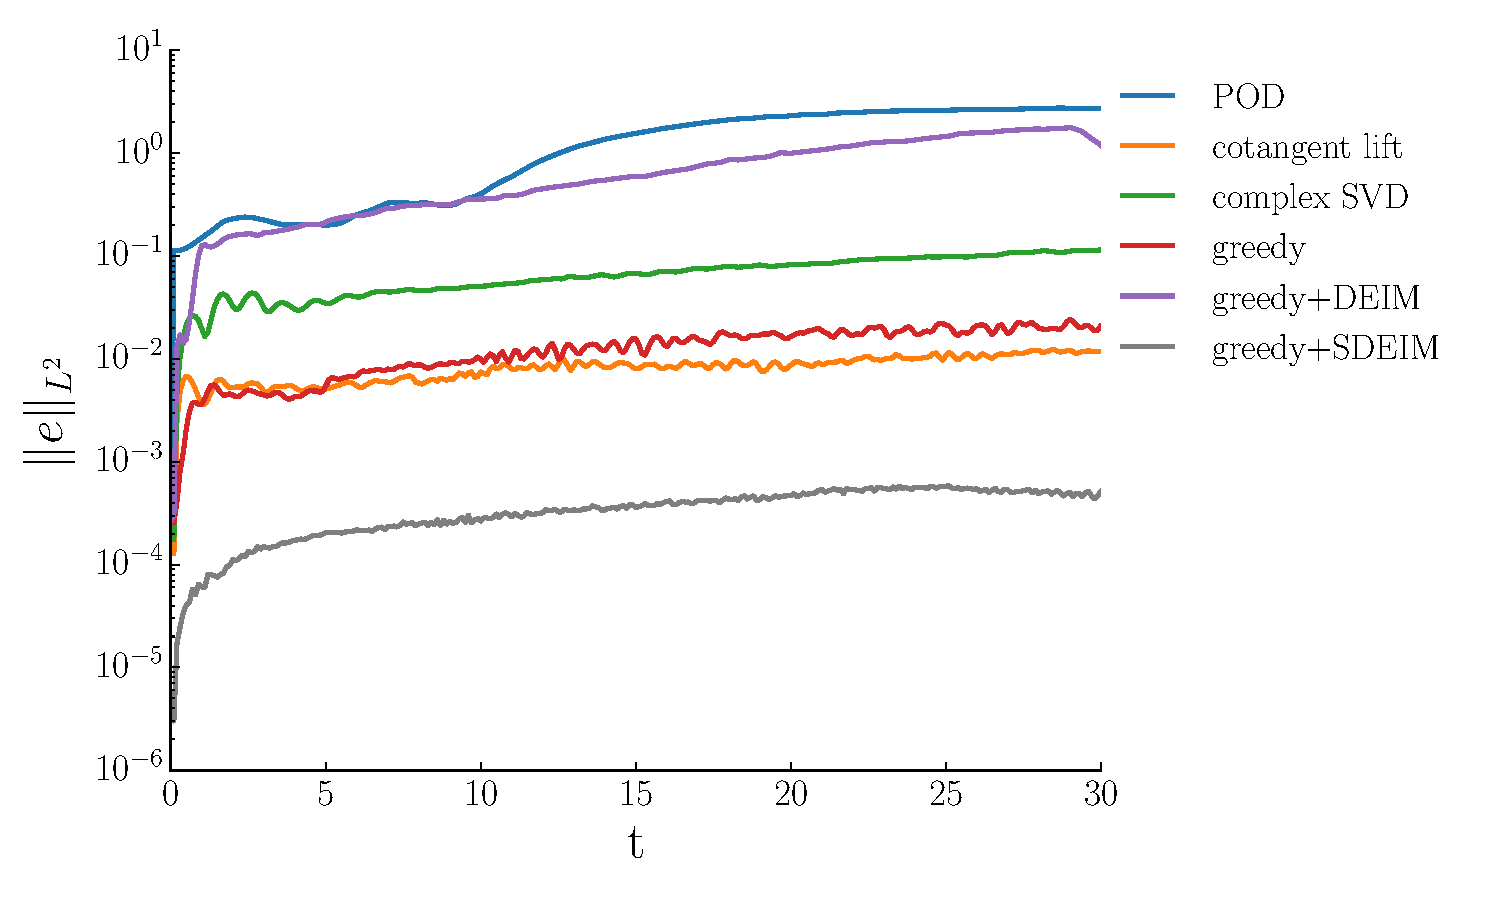
\includegraphics[width=0.5\textwidth]{./figs/schrodinger/error} \\
%	(c)
%\end{tabular}
%\end{center}
%\caption{(a) The decay of singular values for POD, cotangent lift and complex SVD methods. (b) The $L^2$ error between the solution of th full system and the reduced system for different model reduction methods for $t \in [0,30]$. (c) Plot of the Hamiltonian function for $t \in [0,30]$.}\label{fig:NuRe:2}
%\end{figure}

  
\begin{figure}

\begin{minipage}{.5\linewidth}
\centering
\subfloat[$t=0$]{\label{fig:NuRe:3a}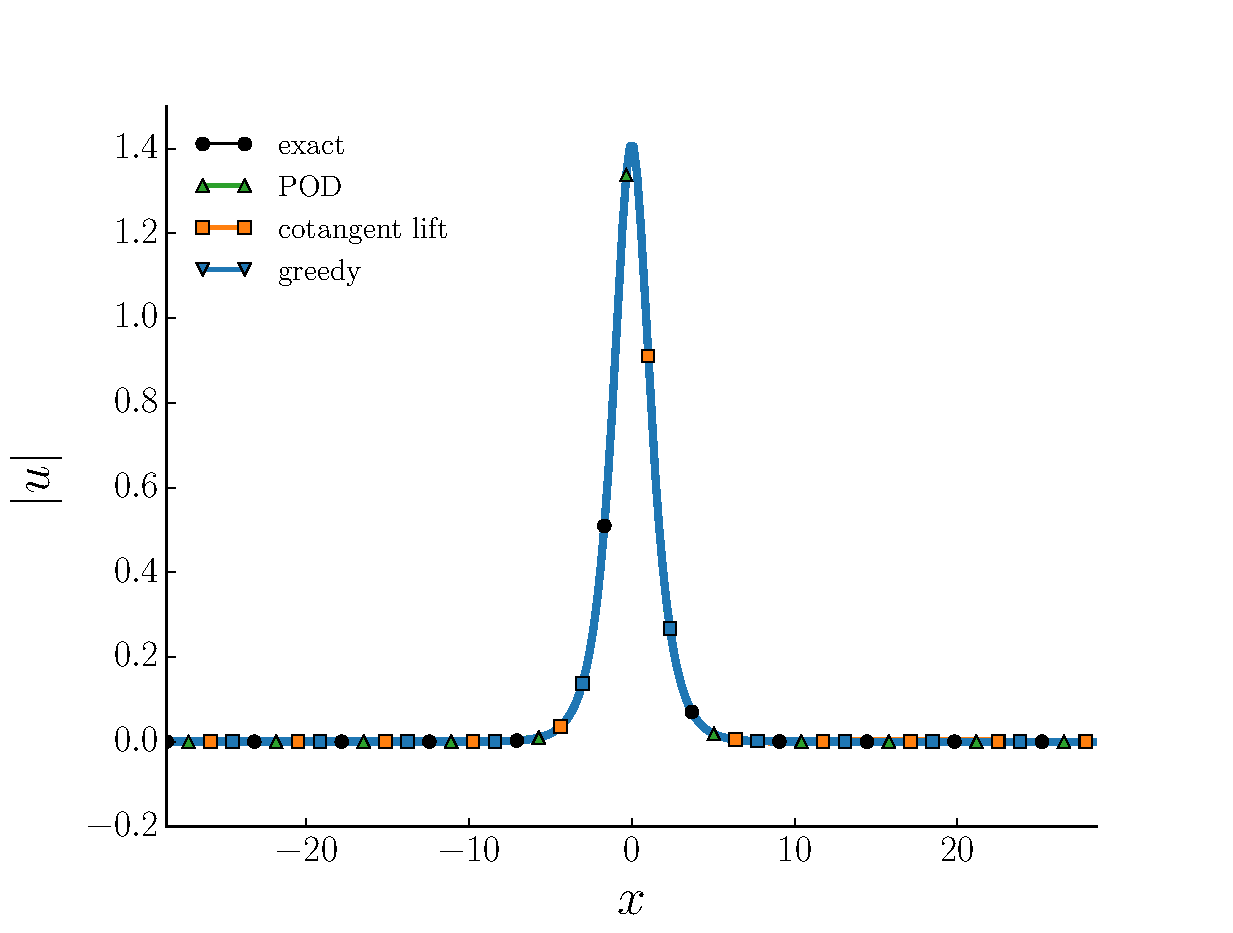
\includegraphics[width=1\textwidth]{./figs/schrodinger/solution/solution_t0}}
\end{minipage}%
\begin{minipage}{.5\linewidth}
\centering
\subfloat[$t=1$]{\label{fig:NuRe:3b}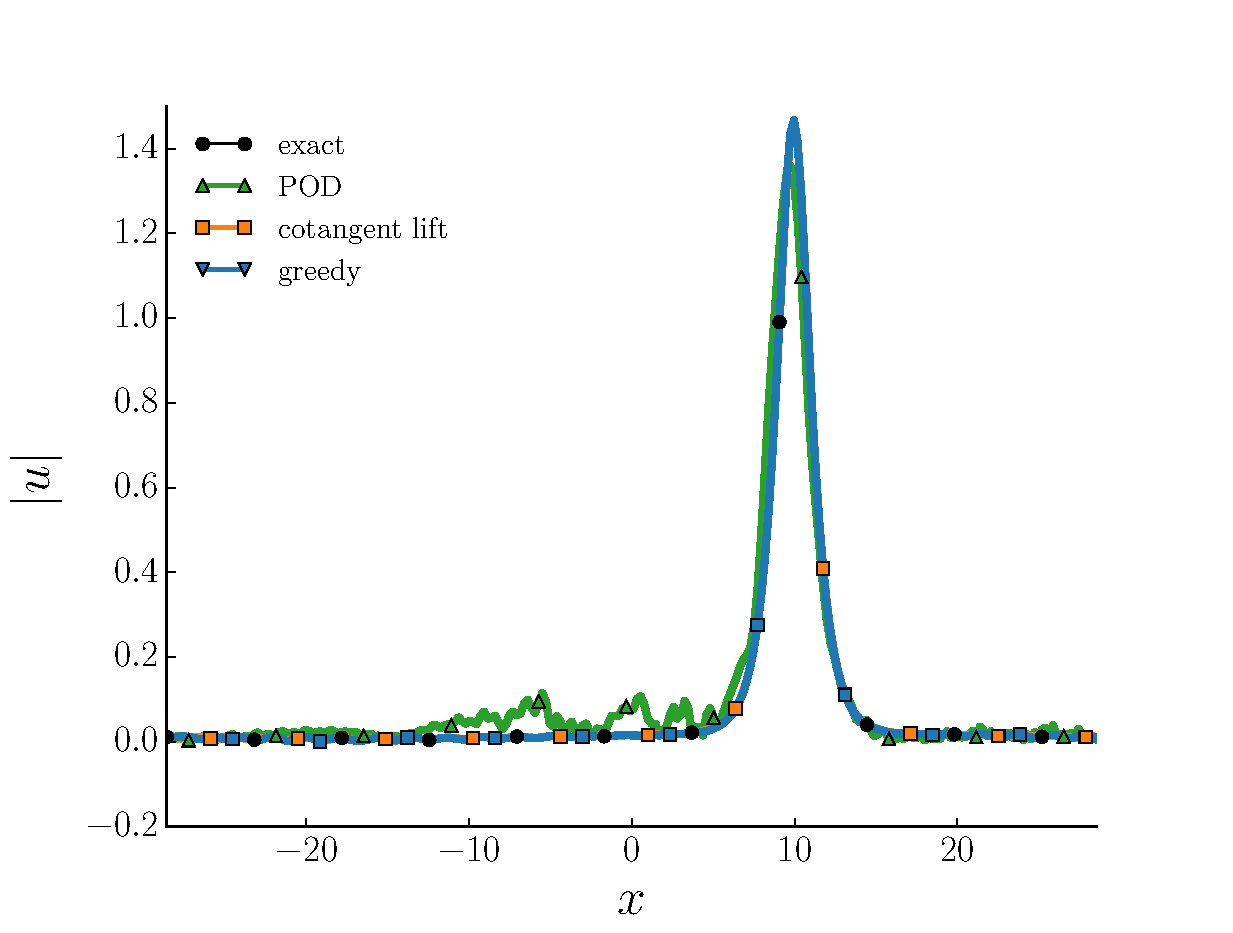
\includegraphics[width=\textwidth]{./figs/schrodinger/solution/solution_t10}}
\end{minipage}\par\medskip
\centering
\subfloat[$t=2$]{\label{fig:NuRe:3c}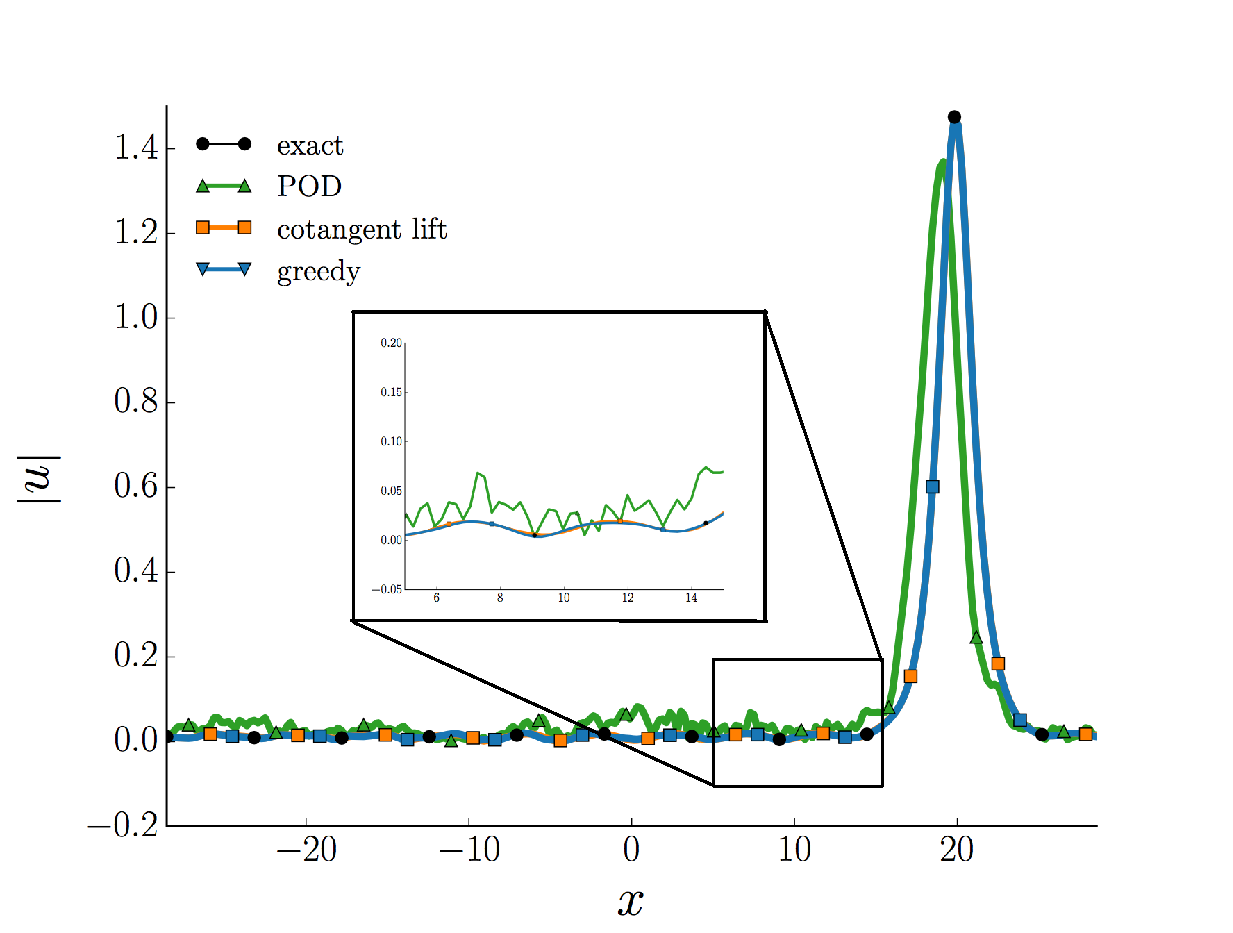
\includegraphics[width=0.5\textwidth]{./figs/schrodinger/solution/solution_t20}}
\caption{The solution $|u(t,x)| = \sqrt{q^2 + p^2}$ at $t=0$, $t=10$ and $t=20$ of the Nonlinear Schr\"odinger equation for parameter value $\epsilon = 1.0932$. Here the solution of {\edit the} full system together with the solution of the POD, cotangent lift, complex SVD and the greedy reduced system is presented.}
\label{fig:NuRe:3}
\end{figure}

\begin{figure}

\begin{minipage}{.5\linewidth}
\centering
\subfloat[]{\label{fig:NuRe:4c}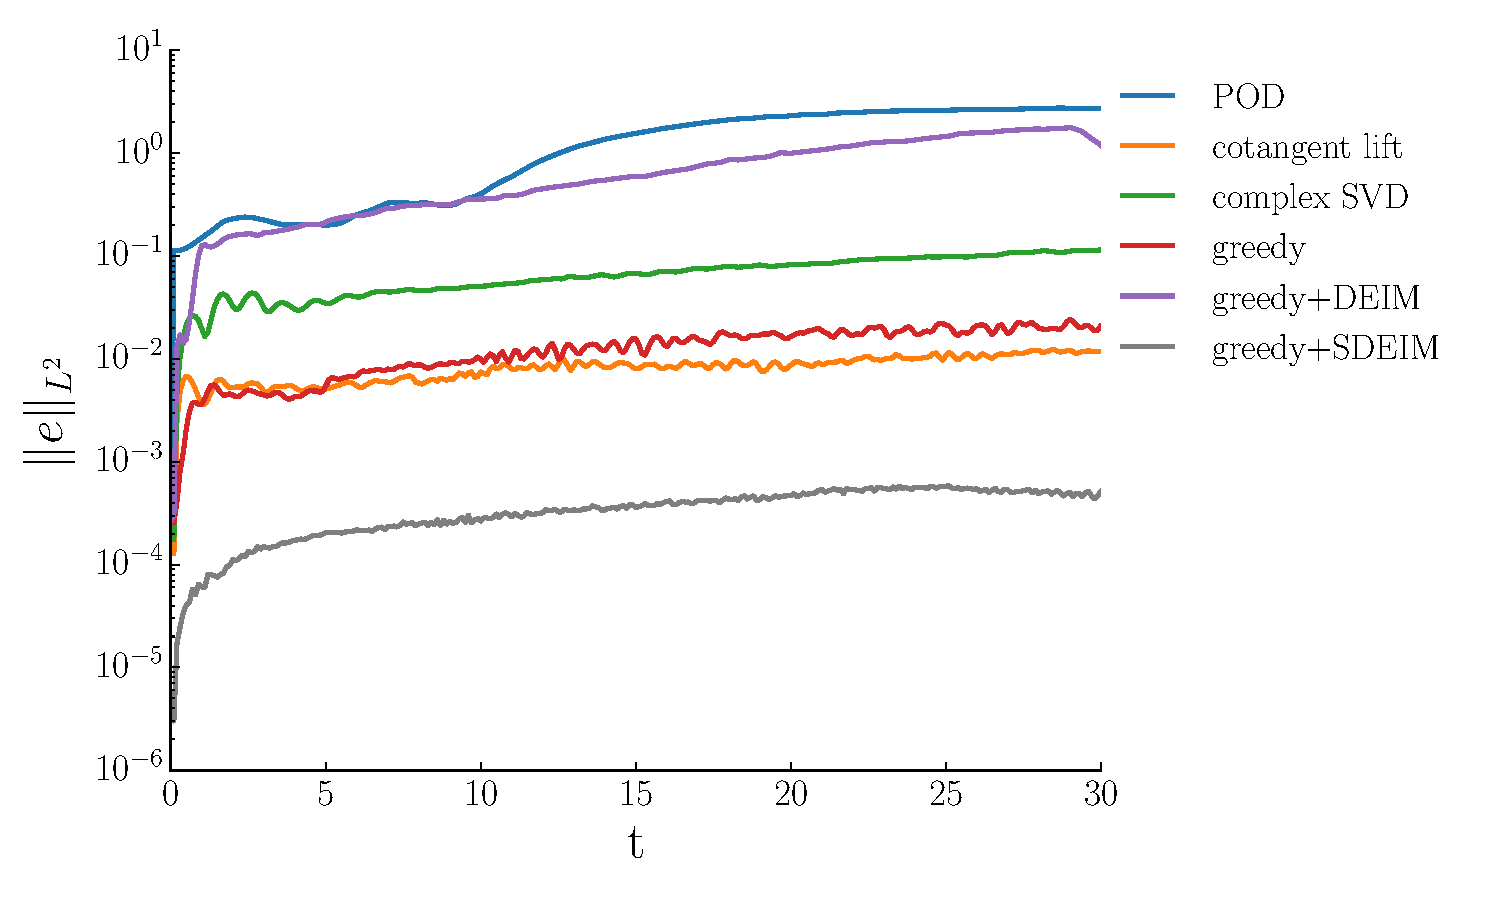
\includegraphics[width=\textwidth]{./figs/schrodinger/error}}
\end{minipage}%
\begin{minipage}{.5\linewidth}
\centering
\subfloat[]{\label{fig:NuRe:4b}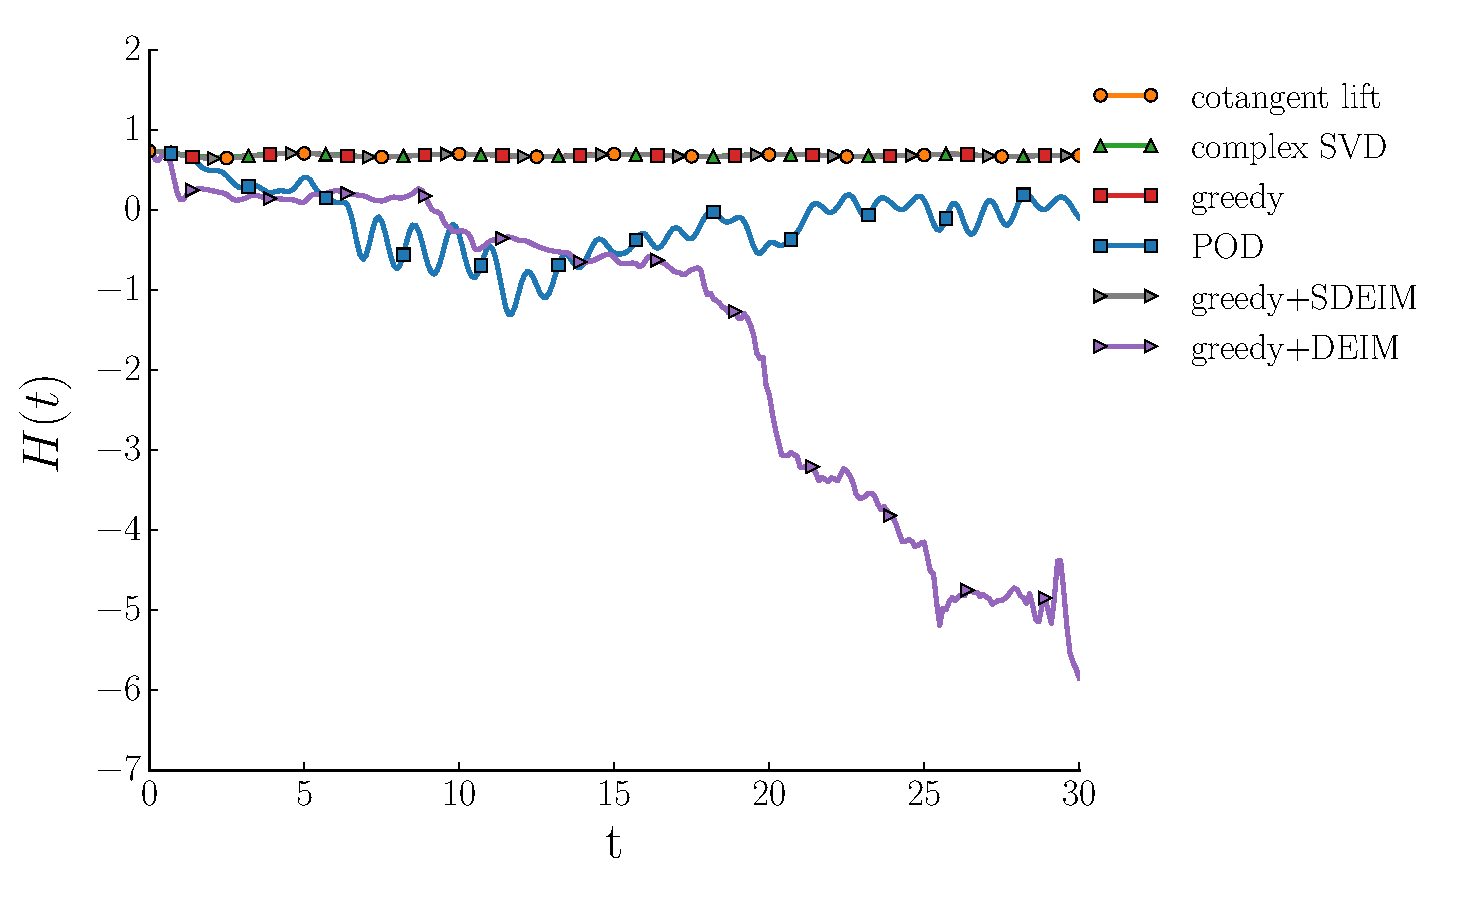
\includegraphics[width=\textwidth]{./figs/schrodinger/hamiltonian}}
\end{minipage}\par\medskip
\centering
%\subfloat[]{\label{fig:NuRe:4c}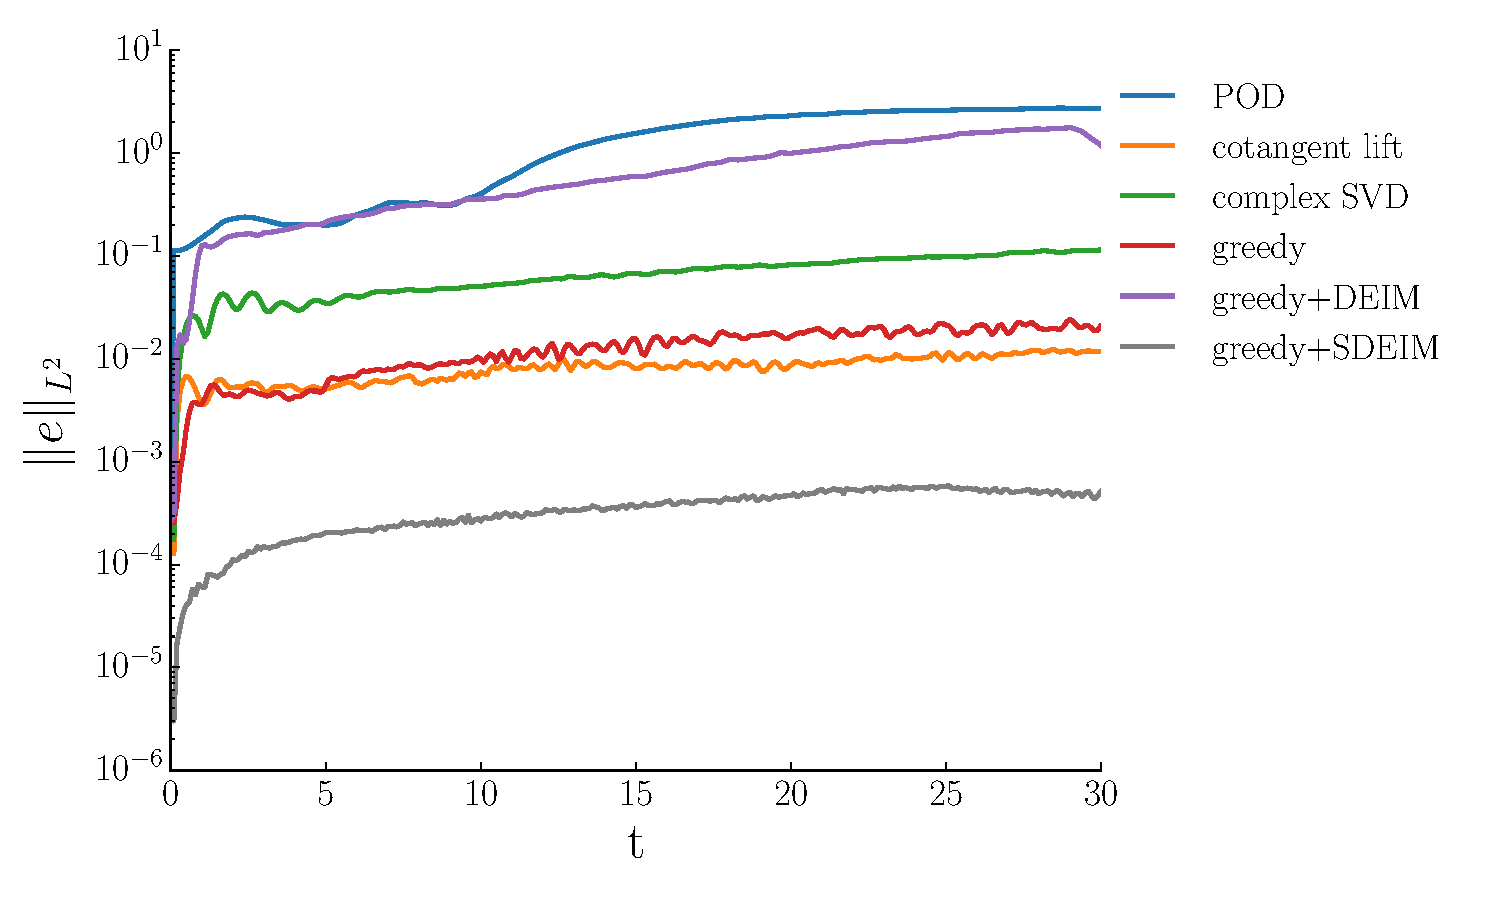
\includegraphics[width=0.5\textwidth]{./figs/schrodinger/error}}

\caption{(a) The decay of singular values for POD, cotangent lift and complex SVD methods. (b) The $L^2$ error between the solution of the full system and the reduced system for different model reduction methods for $t \in [0,30]$. (c) Plot of the Hamiltonian function for $t \in [0,30]$.}
\label{fig:NuRe:4}
\end{figure}


Figure \ref{fig:NuRe:3} shows the solution of the Schr\"odinger equation for parameter value $\epsilon = 1.0932$ at $t=0$, $t=10$ and $t=20$. We first compare the reduced system obtained by the greedy algorithm with POD, cotangent lift and the complex SVD method. The size of the reduced systems are taken identical for all methods ($k=180$ for POD and $k=90$ for the rest). Although the decay of the singular values in Figure \ref{fig:NuRe:4a} suggests that the accuracy of the POD reduced system should be comparable to that of the other methods, we observe instabilities in the solution at $t=10$. The greedy, the cotangent lift and the complex SVD method, on the other hand, generate a stable reduced system that accurately approximates the solution of the full model.

{\edit In Figure \ref{fig:NuRe:4b} we observe that the symplectic methods preserve the Hamiltonian function, unlike the POD and the DIEM methods. We would like to emphasise that using the reduced basis by the greedy and together with the DEIM (purple line) does not preserve the symplectic structure as suggested in this figure.}

Figure \ref{fig:NuRe:4c} illustrates the $L^2$-error between the solution of the full model with the reduced systems generated by different methods. We first observe that symplectic methods yield a lower computational error compared to non-symplectic methods. Secondly, we observe that although the reduced systems from the cotangent lift and the complex SVD are of the same size, their accuracy is different by an order of magnitude. We notice that the greedy algorithm is slightly less accurate than the cotangent lift method while its offline computational cost is less than 20\% {\edit compared to the cotangent lift}. Lastly we notice that the combination of the greedy reduced basis and DEIM yields large errors in the solution while the solution using the symplectic DEIM is very accurate. We note that the symplectic DEIM is even more accurate than the greedy itself since it has been enriched by the nonlinear snapshots. 




